% !TEX program = xelatex
\documentclass[UTF8,a4paper,11pt,fontset=fandol]{ctexart}
\usepackage[left=25mm,right=23mm,top=25mm,bottom=24mm,headheight=16pt]{geometry}
\usepackage{amsmath,amssymb,booktabs,tabularx,longtable,array,multirow}
\usepackage{graphicx,float,xcolor,caption,enumitem,fancyhdr,setspace}
\usepackage{listings,xurl,hyperref,tikz}
\usetikzlibrary{positioning,arrows.meta,fit,calc}
\definecolor{forest}{HTML}{294C3B}
\definecolor{ink}{HTML}{26332C}
\definecolor{muted}{HTML}{687368}
\definecolor{paperline}{HTML}{D9DFD2}
\hypersetup{colorlinks=true,linkcolor=forest,citecolor=forest,urlcolor=forest,
 pdftitle={墒策：可信需水预测与灌溉决策——技术方案},pdfauthor={得分队（AIC-2026-54247845）},bookmarksnumbered=true}
\setstretch{1.20}
\setlength{\parindent}{2em}
\setlength{\parskip}{.15em}
\setlength{\emergencystretch}{2em}
\ctexset{section={format=\Large\bfseries\color{forest},beforeskip=1.2em,afterskip=.8em},
 subsection={format=\large\bfseries\color{forest},beforeskip=1em,afterskip=.5em},
 subsubsection={format=\normalsize\bfseries,beforeskip=.8em,afterskip=.4em}}
\captionsetup{font=small,labelfont=bf,skip=7pt}
\setlist{nosep,leftmargin=2em}
\renewcommand{\arraystretch}{1.22}
\pagestyle{fancy}\fancyhf{}
\fancyhead[L]{\small\color{muted}墒策\quad 技术方案}
\fancyhead[R]{\small\color{muted}AI＋农业}
\fancyfoot[C]{\small\thepage}
\renewcommand{\headrulewidth}{.3pt}
\newcommand{\ET}{\mathrm{ET}_{0}}
\newcommand{\MAE}{\operatorname{MAE}}
\newcommand{\RMSE}{\operatorname{RMSE}}
\newcommand{\clip}{\operatorname{clip}}
\newcommand{\file}[1]{\texttt{\small\path{#1}}}
\newcommand{\datafigure}[4][.94]{\begin{figure}[H]\centering\includegraphics[width=#1\linewidth]{figures/#2}\caption{#3}\label{#4}\end{figure}}
\newcommand{\datatable}[4]{\begin{table}[H]\centering\small\caption{#2}\label{#3}\input{tables/#1}\par\vspace{4pt}{\footnotesize\color{muted}#4}\end{table}}
\lstset{basicstyle=\ttfamily\footnotesize,breaklines=true,columns=fullflexible,
 frame=single,rulecolor=\color{paperline},backgroundcolor=\color{white},showstringspaces=false}
\begin{document}
\begin{titlepage}
\thispagestyle{empty}
\setlength{\parindent}{0pt}
\vspace*{8mm}
\begin{center}
{\Large 2026年第八届\par\vspace{2mm}全球校园人工智能算法精英大赛\par}
\vspace{6mm}{\LARGE\bfseries 算法主题赛\quad AI＋农业\par}
\vspace{4mm}{\LARGE 技术方案\par}
\vspace{14mm}{\color{forest}\rule{.82\linewidth}{1.2pt}\par}
\vspace{10mm}{\fontsize{44}{54}\selectfont\bfseries\color{forest}墒策\par}
\vspace{5mm}{\fontsize{22}{32}\selectfont 可信需水预测与灌溉决策\par}
\vspace{6mm}{\color{muted}\small “墒”取自土壤墒情（根区水分状况），“策”指灌溉决策\par}
\vspace{10mm}{\color{forest}\rule{.82\linewidth}{1.2pt}\par}
\end{center}
\vfill
\begin{center}
\renewcommand{\arraystretch}{1.9}
\begin{tabular}{@{}r@{\quad}l@{}}
\large 团队名称： & \large 得分队\\
\large 团队编号： & \large AIC-2026-54247845\\
\large 赛题名称： & \large AI＋农业\\
\large 作品名称： & \large 墒策：可信需水预测与灌溉决策\\
\end{tabular}
\end{center}
\vspace{16mm}
\begin{center}\large 日期：2026年10月24日\end{center}
\vspace{6mm}
\end{titlepage}
\pagenumbering{Roman}
\section*{摘要}\addcontentsline{toc}{section}{摘要}
华北平原是我国主要的冬小麦—夏玉米产区，也是地下水超采最严重的地区之一，灌溉用水管理直接关系粮食安全与水资源可持续利用。生产中的灌溉决策多依赖经验：一方面难以预判次日作物耗水，另一方面单个天气预测值不包含误差信息，补水时机与补水量难以兼顾。针对这一问题，本作品设计并实现了“墒策”——一个将次日需水预测、预测不确定性量化与根区水量平衡核算连成闭环的灌溉决策系统。作品名中，“墒”指土壤墒情，即根区土壤水分状况；“策”指据此作出的灌溉决策。

在数据层，系统使用Open-Meteo历史天气接口提供的ERA5再分析逐日气象数据，覆盖石家庄、郑州、济南三地2018—2025年，共8766条记录，以目标日前的气温、湿度、风速、降水、短波辐射、地表气压与历史参考蒸散构造49维特征。在模型层，采用直方图梯度提升树回归次日FAO-56参考蒸散（ET\textsubscript{0}），以2018—2022年训练、2023年独立校准、2024—2025年测试，严格按时间隔离；在此基础上用分割式共形方法给出名义90\%预测区间。在决策层，将预测ET\textsubscript{0}与作物系数、土壤总可用水、灌溉效率和日供水上限结合，按FAO-56水量平衡计算是否灌溉以及补多少水，并输出可追溯的决策记录。

在2193条时间留出测试样本上，模型平均绝对误差为0.7757 mm/日，较“沿用昨日值”基线降低7.68\%；均方根误差1.0688 mm/日，决定系数0.7103；90\%预测区间的实际覆盖率为91.06\%。完全留出某一地区的迁移检验中，三地点预测均优于昨日值基线。在三地、两年、三档土壤容量、两档灌溉效率共180组生长季仿真中，基准情景下“区间上界”策略将缺水风险日由墒情阈值策略的9.33日降至0日，季均毛灌溉量377.04 mm，较定额日历灌溉少用31.4\%。诊断分析同时发现，6—7月高需水期区间覆盖率降至约78\%\,$\sim$\,79\%，据此提出分季节校准的改进方向。

系统已实现历史回放、预测区间展示、土壤参数交互、供水能力检查和决策记录导出，代码、数据、模型与逐日结果全部可复现。本作品为灌溉方法教学、农技分析和试点前评估提供了一套可检验的工具，下一步将接入实时气象预报与田间墒情观测开展影子运行。

\vspace{5mm}\noindent\textbf{关键词：}参考蒸散；梯度提升树；共形预测；根区水量平衡；灌溉决策；墒情
\clearpage
\setcounter{tocdepth}{2}
\begingroup\setstretch{1}\fontsize{9.5}{10.5}\selectfont\setlength{\parskip}{0pt}\tableofcontents\endgroup
\clearpage\pagenumbering{arabic}
\section{作品概述}
\subsection{背景介绍}
农业是我国第一用水大户，灌溉用水效率的提升是节水型社会建设的关键环节。华北平原集中了冬小麦—夏玉米一年两熟的主要产区，降水年内分配不均，春季与初夏的作物需水高峰往往与少雨期重叠，灌溉高度依赖地下水，长期超采已形成大范围地下水漏斗。在这一背景下，“什么时候灌、灌多少”不再只是农事经验问题，而是同时关系粮食稳产与水资源可持续利用的管理问题。

国际上通行的灌溉决策框架以FAO-56为代表：先由气象条件计算参考蒸散ET\textsubscript{0}，再乘以作物系数得到作物需水，结合根区土壤水量平衡判断是否需要补水\cite{fao,pereira}。这一框架机理清晰，但在基层落地时面临两点困难：其一，决策需要的是\emph{次日}乃至未来几天的需水，而不是已经发生的蒸散；其二，任何预测都有误差，单一预测值无法告诉使用者“如果预测偏低会怎样”。经验灌溉往往通过多灌来对冲不确定性，造成水资源浪费和深层渗漏；按平均值精确灌溉，又可能在需水突增时出现缺水胁迫\cite{fereres}。

近年来，机器学习方法在日参考蒸散估算与预测上取得了较多进展。随机森林、梯度提升树等集成方法在中国不同气候区的ET\textsubscript{0}建模中表现稳定，在气象输入不完整时也能保持较好精度\cite{fan,feng}。但已有工作大多止步于“预测精度”，较少回答两个与灌溉直接相关的问题：预测误差有多大、能否被量化；预测结果进入灌溉规则后，用水量与缺水风险如何变化。这正是本作品切入的位置。

\subsection{作品名称释义}
作品命名为“墒策”。“墒”（shāng）是我国传统农业术语，指土壤中适宜作物生长的水分状况，生产上常说“看墒情”“保墒”“抢墒播种”，各级农业部门也长期开展土壤墒情监测。“策”指决策。墒策即“依墒情定灌溉之策”：系统以根区土壤水分亏缺为核心状态量，把次日需水预测及其误差区间转化为具体的补水建议。副标题“可信需水预测与灌溉决策”中的“可信”，指预测结果附带经独立年份校准的误差区间，并且每一条建议都能追溯到输入数据、模型版本和计算过程。

\subsection{目标定位}
本作品的目标是构建一个面向农技人员与农业信息化教学的灌溉决策工具，具体包括：
\begin{enumerate}
\item \textbf{次日需水预测}：仅使用目标日前已发生的气象数据，预测次日参考蒸散，精度优于“沿用昨日值”这一业务上常用的简单基线；
\item \textbf{误差可量化}：为每个预测给出名义90\%的预测区间，并在未参与训练的年份上检验其实际覆盖率；
\item \textbf{预测进入决策}：将预测值或区间上界代入FAO-56根区水量平衡，计算是否灌溉、毛灌溉量、净补水量，并显式检查日供水能力；
\item \textbf{策略可比较}：在统一的气象与土壤情景下，比较定额日历、墒情阈值、昨日值预测、AI点预测与AI区间上界五种策略的用水量与缺水风险；
\item \textbf{过程可追溯}：交互界面、服务端计算与导出记录保持一致，全部结果能由原始数据和脚本重现。
\end{enumerate}

\subsection{技术路线与系统组成}
图\ref{fig:arch}给出系统的整体结构。系统分为数据层、预测层、决策层和交互层：数据层获取并校验三地公开气象序列；预测层构造49维历史特征，训练梯度提升树并在独立年份校准误差区间；决策层将参考蒸散乘以作物系数，计入根区亏缺，并在供水上限约束下计算补水量；交互层以图谱形式展示需水曲线、预测区间、根区水量和建议结果，并支持导出决策记录。

\begin{figure}[H]\centering
\begin{tikzpicture}[font=\small,
 box/.style={draw=forest,line width=.8pt,rounded corners=2pt,fill=white,align=center,minimum height=12mm,minimum width=27mm,inner xsep=3mm},
 layer/.style={fill=forest!8,draw=none,rounded corners=3pt},
 arr/.style={-{Stealth[length=2.4mm]},line width=.8pt,color=forest}]
\node[box] (d) {数据层\\[1pt]\footnotesize ERA5逐日气象\\\footnotesize 校验与归档};
\node[box,right=8mm of d] (m) {预测层\\[1pt]\footnotesize 49维特征\\\footnotesize 梯度提升树};
\node[box,right=8mm of m] (c) {不确定性\\[1pt]\footnotesize 2023年独立校准\\\footnotesize 90\%预测区间};
\node[box,right=8mm of c] (w) {决策层\\[1pt]\footnotesize FAO-56水量平衡\\\footnotesize 供水能力约束};
\node[box,below=10mm of m] (u) {交互层\\[1pt]\footnotesize 历史回放 · 参数调节 · 记录导出};
\node[box,below=10mm of w] (s) {策略仿真\\[1pt]\footnotesize 5种策略×36个情景};
\draw[arr] (d)--(m); \draw[arr] (m)--(c); \draw[arr] (c)--(w);
\draw[arr] (w.south)--(s.north);
\draw[arr] (w.south west)--(u.north east);
\draw[arr] (m.south)--(u.north);
\end{tikzpicture}
\caption{墒策系统结构与数据流}\label{fig:arch}
\end{figure}

\subsection{作品特色与创新点}
\textbf{（1）把预测误差放进灌溉决策。}多数需水预测工作只报告点预测精度。本作品用分割式共形方法在独立年份上校准误差分位数\cite{vovk,lei}，将区间上界作为“保守需水”直接代入灌溉触发规则，使使用者能够在“少用水”和“少缺水”之间作出知情选择，而不是被动接受一个数字。

\textbf{（2）机理模型与数据驱动方法耦合。}预测部分采用数据驱动的梯度提升树，决策部分严格遵循FAO-56的作物系数与根区水量平衡框架。模型只负责其擅长的短期气象需水预测，土壤、作物与设备约束由可解释的机理公式处理，二者通过作物系数与亏缺状态衔接，符合赛题倡导的“机理—数据耦合建模”。

\textbf{（3）供水能力显式建模。}当建议补水量超过设备或水源的日供水上限时，系统按上限给出可执行的补水量，同时提示能力不足与补水后的预计亏缺，而不是悄悄截断、营造“已满足需水”的假象。这一设计贴近灌区轮灌、机井出水量受限等实际约束。

\textbf{（4）严格的时间隔离与全链条可复现。}特征只使用目标日前的数据，训练、校准、测试按年份切分，并以自动化测试验证“扰动目标日及之后数据不改变输入特征”。原始接口响应、模型文件、逐日预测与180组仿真明细随工程交付，主要指标均可由脚本从CSV重算。

\textbf{（5）正负结果同时报告。}作品不仅给出整体指标，还按月份、地区和极端误差样本做了诊断，发现夏季高需水期区间覆盖不足等问题，并据此提出改进路线，使评估结论更可靠，也为后续优化指明了方向。

\section{需求分析}
\subsection{问题剖析}
灌溉决策的本质是在不确定条件下对“补水时机”和“补水量”作出选择。围绕这一问题，可以从以下四个维度分析其难点。

\textbf{需水的时间维度。}作物耗水由当天的辐射、温度、湿度与风速共同决定，具有明显的季节性和日际波动。在华北，5—7月参考蒸散可达每日6\,$\sim$\,9 mm，一次天气转折就可能使次日需水成倍变化。依据“昨天耗多少、今天补多少”的经验做法，在天气突变时会明显滞后。

\textbf{土壤的状态维度。}同样的次日需水，对根区水分充足的地块意味着无需灌溉，对接近胁迫阈值的地块则必须补水。因此，需水预测必须与根区水分亏缺一起使用，单看天气无法得出灌溉结论。FAO-56以“总可用水TAW—易利用水RAW—当前亏缺”描述这一状态，是业内通行的方法\cite{fao}。

\textbf{误差的风险维度。}预测偏低会推迟补水，造成作物水分胁迫；预测偏高会提前补水，增加无效用水和深层渗漏。两类错误的后果不对称，且与土壤缓冲能力、供水条件相关。只给出一个点预测，使用者无法判断风险大小，也就无法根据自身情况选择保守或节水的策略。

\textbf{约束的执行维度。}实际灌溉受机井出水量、管网压力、轮灌时段和劳动力等条件限制，计算出的“理论需水”未必能当天补足。若系统忽略供水能力，给出的建议可能无法执行，或让使用者误以为需水已经满足。

综合来看，核心痛点不在于缺少某一个预测模型，而在于“预测—误差—土壤—设备”之间缺少一条贯通、可检查的链条。这是本作品要解决的关键问题。

\subsection{需求调研}
本作品的需求调研以文献研究、公开数据分析和原型迭代三种方式开展。

\textbf{文献研究。}梳理FAO-56及其后续修订工作\cite{fao,pereira}，明确参考蒸散、作物系数、根区水量平衡和触发阈值的标准定义；调研亏缺灌溉相关研究\cite{fereres}与AquaCrop作物模型\cite{aquacrop}，明确水分胁迫与产量响应之间的关系及其所需的田间参数；调研国内ET\textsubscript{0}机器学习预测研究\cite{fan,feng}，确定树集成模型在有限气象输入下的适用性与常用评价指标。

\textbf{公开数据分析。}对三地2018—2025年逐日气象进行统计（图\ref{fig:climate}），确认参考蒸散在5—7月达到峰值、降水集中于7—8月，需水高峰与降水高峰存在错位。这说明春夏之交是灌溉决策压力最大、预测价值最高的时段，也决定了后续诊断要重点检查夏季月份的表现。

\textbf{原型迭代。}以典型使用流程为线索搭建原型，围绕“输入什么、看到什么、导出什么”多轮调整界面与接口。例如，早期版本只显示建议量，迭代后增加了“补水后预计亏缺”和“供水能力不足”提示；为防止页面状态与导出记录不一致，增加了服务端重算与请求编号校验。

在此基础上，确定目标用户为两类：一是需要比较不同灌溉情景、向农户提供建议的基层农技人员；二是农业水利、农业信息化相关课程的教师和学生。典型工作流程为：选择地区与日期，查看次日需水预测、误差区间和昨日值基线；输入当前根区亏缺、土壤总可用水、作物系数、灌溉效率和日供水上限；系统给出是否灌溉、毛灌溉量、净补水量与依据；使用者确认后导出本次决策记录，供后续复核。

\subsection{功能需求}
\begin{table}[H]\centering\small
\caption{功能需求与验收方式}\label{tab:requirements}
\begin{tabularx}{\linewidth}{@{}p{.18\linewidth}XX@{}}\toprule
需求 & 实现内容 & 验收方式\\\midrule
次日需水预测 & 基于目标日前49维特征推理次日ET\textsubscript{0} & 时间留出测试MAE优于昨日值基线\\
误差区间展示 & 曲线叠加名义90\%预测区间 & 独立年份校准，测试期检验覆盖率\\
基线对照 & 同屏显示昨日值与事后参考值 & 参考值仅用于核验，不进入模型输入\\
根区水量核算 & 显示剩余可用水、亏缺与触发线 & 参数变化时图形与计算同步更新\\
灌溉建议 & 输出毛灌溉量、净补水量与依据 & 与独立公式实现逐项一致\\
供水能力检查 & 建议量不超过日供水上限并提示 & 极小上限触发能力不足提示\\
记录导出 & JSON保存参数、策略、模型版本与结果 & 导出内容与页面当前输入一致\\
异常处理 & 非法参数、日期、地区返回错误 & 错误状态下禁止导出，修正后可恢复\\\bottomrule
\end{tabularx}
\end{table}

\subsection{非功能需求}
\begin{table}[H]\centering\small
\caption{非功能需求与实现方式}\label{tab:nonfunc}
\begin{tabularx}{\linewidth}{@{}p{.18\linewidth}X@{}}\toprule
维度 & 实现方式\\\midrule
可解释性 & 阈值、回填目标、效率与上限均以显式公式计算，界面同步展示依据\\
可复现性 & 保留原始接口响应与SHA-256哈希，固定依赖版本与随机种子\\
离线可用 & 模型、数据和页面部署在同一台计算机，推理不依赖外部服务\\
轻量部署 & 模型文件约416 KiB，单次推理中位耗时约11.5 ms，普通笔记本即可运行\\
数据安全 & 服务仅监听本机回环地址，不采集用户身份信息\\
跨端适配 & 手机竖屏布局适配，无横向溢出（局域网访问需另行配置服务地址）\\\bottomrule
\end{tabularx}
\end{table}

\subsection{评价指标设计}
预测精度、用水量和缺水风险是相互关联又彼此冲突的目标：更高的需水估计能降低缺水风险，却会增加用水；更低的估计则相反。为避免用任意加权的“综合得分”掩盖这一权衡，本作品分层评价：

\begin{itemize}
\item \textbf{模型层}：平均绝对误差MAE、均方根误差RMSE、决定系数$R^2$，以及预测区间的经验覆盖率与平均宽度；
\item \textbf{决策层}：季节毛灌溉量、缺水风险日（日末亏缺超过RAW的天数）、排水量和未满足需水量；
\item \textbf{系统层}：服务端参数校验、导出一致性、异常恢复与移动端适配。
\end{itemize}

这种分层设计使每一项结论都能对应到具体的数据与检验，也便于在接入田间数据后逐层替换和扩展。

\clearpage\section{AI技术工具选择与运用}
\subsection{技术选型总览}
本作品为团队自行研发的软件系统，核心AI技术为基于梯度提升决策树的次日参考蒸散回归，以及基于分割式共形预测的不确定性量化。表\ref{tab:stack}列出主要技术与工具及其选型依据。

\begin{table}[H]\centering\small
\caption{主要技术、工具与选型依据}\label{tab:stack}
\begin{tabularx}{\linewidth}{@{}p{.20\linewidth}p{.25\linewidth}X@{}}\toprule
环节 & 技术/工具 & 选型依据\\\midrule
气象数据 & Open-Meteo历史接口（ERA5） & 覆盖全国、逐日连续、字段齐全，含FAO-56参考蒸散，CC BY 4.0许可\\
特征工程 & pandas 2.3 & 按地区分组的滞后与滚动窗口计算，便于保证时间边界\\
预测模型 & scikit-learn 1.7 梯度提升树（\texttt{\small HistGBR}） & 擅长中小规模结构化数据与非线性关系，CPU训练快，模型小\\
不确定性 & 分割式共形预测 & 不依赖误差分布假设，实现简单，可在独立年份上校准\\
决策规则 & FAO-56水量平衡 & 国际通行的灌溉计算框架，参数物理意义明确\\
交互系统 & Python HTTP服务＋原生HTML/JS & 无需额外框架，离线可运行，便于部署到基层电脑\\
测试 & pytest、Playwright & 覆盖计算逻辑与浏览器端交互\\\bottomrule
\end{tabularx}
\end{table}

\subsection{数据来源与质量控制}
数据通过Open-Meteo历史天气接口获取\cite{om}，模式设为ERA5，时区为Asia/Shanghai，风速单位m/s，时间范围2018年1月1日至2025年12月31日。ERA5是欧洲中期天气预报中心发布的第五代全球再分析产品，将多源观测同化进数值模式，重建逐时大气状态\cite{era5}。选取华北平原及邻近的石家庄、郑州、济南三地作为示范点，它们分别代表冀中、豫中和鲁中的主要粮食产区。

\begin{table}[H]\centering\small
\caption{示范地点与接口返回网格}\label{tab:sites}
\begin{tabular}{lrrrrr}\toprule
地点 & 请求纬度 & 请求经度 & 网格纬度 & 网格经度 & 原始日数\\\midrule
石家庄 & 38.04 & 114.51 & 38.00 & 114.50 & 2922\\
郑州 & 34.75 & 113.62 & 34.75 & 113.50 & 2922\\
济南 & 36.65 & 117.12 & 36.75 & 117.00 & 2922\\\bottomrule
\end{tabular}
\end{table}

原始JSON完整保留返回坐标、海拔、字段单位与逐日数组，并记录请求URL、获取时间和SHA-256哈希。表\ref{tab:variables}列出所用变量。

\begin{table}[H]\centering\small
\caption{原始变量、单位与使用方式}\label{tab:variables}
\begin{tabularx}{\linewidth}{@{}p{.25\linewidth}p{.18\linewidth}X@{}}\toprule
变量 & 单位 & 用途\\\midrule
平均、最高、最低气温 & $^\circ$C & 历史滞后值与7日均值\\
平均相对湿度 & \% & 历史湿度状态\\
10米高度风速 & m/s & 历史风速特征\\
日降水量 & mm & 历史特征；目标日降水仅用于仿真中的日末水量更新\\
短波辐射日总量 & MJ/m$^2$ & 历史能量条件\\
地表平均气压 & hPa & 历史特征\\
参考蒸散ET\textsubscript{0} & mm/日 & 历史特征与预测目标\\\bottomrule
\end{tabularx}
\end{table}

读入阶段按完整日历重建索引，逐项检查：最高气温不低于最低气温，相对湿度位于0\,$\sim$\,100\%，风速、降水与参考蒸散非负，并屏蔽可能的缺测码。三地关键字段均无缺失，未做任何插补。

\subsection{预测目标与季节结构}
图\ref{fig:climate}按月汇总全部8766条记录。参考蒸散在5—7月达到峰值，而降水集中在7—8月，春季和初夏是需水与供水矛盾最突出的时段。

\datafigure{climate.pdf}{三地2018—2025年月平均气象概况（降雨为日均毫米）}{fig:climate}

预测目标为FAO-56 Penman--Monteith日参考蒸散\cite{fao}：
\begin{equation}\label{eq:pm}
\mathrm{ET}_0=\frac{0.408\Delta(R_n-G)+\gamma\dfrac{900}{T+273}u_2(e_s-e_a)}{\Delta+\gamma(1+0.34u_2)},
\end{equation}
其中$R_n$为净辐射，$G$为土壤热通量，$T$为日平均气温，$u_2$为2米风速，$e_s-e_a$为饱和水汽压差，$\Delta$为饱和水汽压曲线斜率，$\gamma$为湿度计常数。式\eqref{eq:pm}表明参考蒸散由能量项和空气动力学项共同决定，这也是特征设计中同时纳入辐射、温度、湿度与风速的依据。主实验以接口提供的\texttt{et0\_fao\_evapotranspiration}作为标签，工程中另有一份独立的FAO-56计算函数用于公式和单位核验。

\subsection{特征构造与时间边界}
对地区$s$的目标日$t$，原始变量集合为
\begin{equation}
\mathcal V=\{T_{\rm mean},T_{\max},T_{\min},RH,u_{10},P,R_s,p_a,\mathrm{ET}_0\}.
\end{equation}
对每个$v\in\mathcal V$构造4个滞后值和1个7日均值：
\begin{align}
L_{s,t}^{v,k}&=v_{s,t-k},\qquad k\in\{1,2,3,7\},\\
M_{s,t}^{v,7}&=\frac{1}{7}\sum_{j=1}^{7}v_{s,t-j}.
\end{align}
共$9\times5=45$个历史特征，另加纬度、经度和年内日期$d_t$的周期编码
\begin{equation}
a_t=\sin(2\pi d_t/365.25),\qquad b_t=\cos(2\pi d_t/365.25),
\end{equation}
最终输入$x_{s,t}$为49维。目标日当天的气温、降水、辐射和参考蒸散均不进入输入。

7日窗口按地区独立计算，避免跨地区拼接。实现上先\texttt{shift(1)}再\texttt{rolling(7)}，保证窗口不含目标日。单元测试将目标日及之后的全部气象字段大幅扰动，验证目标日的49维特征保持不变。每地前7天无法形成完整窗口，共删除21条记录。

\subsection{梯度提升树模型}
逐日气象输入是规模有限的结构化数据，变量间存在非线性和阈值效应。梯度提升决策树逐轮拟合损失函数的负梯度，将多棵弱回归树相加\cite{friedman}，在表格数据上表现稳健，XGBoost与LightGBM等实现已被广泛使用\cite{xgb,lgbm}。在国内ET\textsubscript{0}建模研究中，树集成模型也被证明能在有限气象输入下取得较好的精度\cite{fan,feng}。本作品采用scikit-learn的\texttt{HistGradientBoostingRegressor}\cite{sklearn}，其直方图分箱策略与LightGBM类似，在普通CPU上即可完成训练。

以平方误差为学习目标：
\begin{equation}
\widehat f=\arg\min_f\sum_{i\in\mathcal D_{\rm tr}}\tfrac12\bigl(y_i-f(x_i)\bigr)^2+\Omega(f),
\end{equation}
其中$\Omega$为叶节点正则项。迭代形式为
\begin{equation}
f_m(x)=f_{m-1}(x)+\nu h_m(x),\quad m=1,\ldots,M,
\end{equation}
预测值截断为非负。超参数见表\ref{tab:hyper}，全部在接触测试集之前固定。

\begin{table}[H]\centering\small
\caption{模型超参数}\label{tab:hyper}
\begin{tabularx}{\linewidth}{@{}l l X@{}}\toprule
参数 & 取值 & 作用\\\midrule
最大迭代轮数$M$ & 180 & 控制加性模型规模\\
学习率$\nu$ & 0.055 & 控制每棵新树的权重\\
最大叶节点数 & 15 & 限制单树复杂度\\
叶节点最小样本数 & 25 & 防止过细分裂\\
L2正则化 & 8 & 约束叶节点权重\\
内部早停 & 关闭 & 避免随机划分打乱时间顺序\\
随机种子 & 42 & 保证可重复\\
损失函数 & 平方误差 & 连续非负标签回归\\\bottomrule
\end{tabularx}
\end{table}

\subsection{数据划分}
按年份严格切分：2018—2022年为训练集（5457条），2023年为校准集（1095条），2024—2025年为测试集（2193条）。模型只在训练集上拟合，校准集只用于估计误差分位数，测试集不参与任何拟合、校准或调参。图\ref{fig:annual}展示各阶段的年度均值。

\datafigure{annual.pdf}{各地区年度日均参考蒸散与数据分段（阴影为校准年和测试年）}{fig:annual}

\subsection{预测区间的共形校准}
令校准集大小$n_c=1095$，计算每个校准样本的绝对残差
\begin{equation}
r_i=|y_i-\widehat f(x_i)|.
\end{equation}
在名义失覆盖率$\alpha=0.1$下，取有限样本修正的次序统计量\cite{vovk,lei,conformal}
\begin{equation}\label{eq:quantile}
k=\min\{n_c,\lceil(n_c+1)(1-\alpha)\rceil\},\qquad q=r_{(k)}.
\end{equation}
本次$k=987$，$q=1.8506$ mm/日。测试区间为
\begin{equation}\label{eq:interval}
C(x)=\bigl[\max(0,\widehat f(x)-q),\ \widehat f(x)+q\bigr].
\end{equation}
由于参考蒸散非负，下界截断为0，因此低预测值处的区间宽度小于$2q$。共形预测的理论覆盖保证以样本可交换为前提，而气象序列存在时间相关和季节漂移，因此本作品在测试期逐月、逐地区检验经验覆盖率（第\ref{sec:results}章），而不是直接套用理论保证。

\subsection{对照方法与迁移检验}
为分离季节信息、近期天气信息和历史蒸散的贡献，设置四种对照：
\begin{itemize}
\item \textbf{地区月均值}：用训练年份中各地区各月的ET\textsubscript{0}均值作预测；
\item \textbf{昨日值}：$\widehat y_t=y_{t-1}$，业务中最常用的持续性预测；
\item \textbf{日期与位置}：同类梯度提升树，仅输入周期日期与经纬度4个特征；
\item \textbf{去除历史蒸散}：保留近期天气特征，去掉全部历史ET\textsubscript{0}特征（消融实验）。
\end{itemize}
所有方法在同一2193条测试样本上评价。

跨地区迁移检验另行训练三次模型，每次彻底排除一个地区的训练和校准数据：在另外两地2018—2022年拟合，用另外两地2023年残差校准，再在留出地区2024—2025年测试，用于评估模型推广到未见地区的能力。

\clearpage\section{项目实施}
\subsection{实施方案设计}
\subsubsection{实施步骤}
项目按“数据—模型—决策—系统—评估”五个阶段推进，每个阶段都设置可检验的产出，前一阶段验收后再进入下一阶段。

\begin{table}[H]\centering\small
\caption{实施步骤与阶段产出}\label{tab:plan}
\begin{tabularx}{\linewidth}{@{}p{.15\linewidth}XX@{}}\toprule
阶段 & 主要工作 & 验收产出\\\midrule
数据准备 & 选点、调用接口、保存原始响应、质量检查 & 三地原始JSON与哈希清单，缺失与范围检查记录\\
模型构建 & 特征工程、时间划分、模型训练、共形校准 & 已训练模型、特征列表、校准分位数\\
决策规则 & 作物系数情景、水量平衡与供水约束实现 & 规则函数与独立公式核验测试\\
系统开发 & 推理接口、交互界面、记录导出 & 本地可运行的决策工作台\\
评估与诊断 & 时间留出测试、迁移检验、180组仿真 & 逐日预测、仿真明细、诊断图表与本报告\\\bottomrule
\end{tabularx}
\end{table}

\subsubsection{资源配置}
项目全部基于开源工具与公开数据完成。软件环境为Python 3.12及NumPy、pandas、scikit-learn、Matplotlib等库，界面使用浏览器原生HTML、CSS与JavaScript；硬件为普通笔记本电脑，训练与推理均在CPU上完成，无需GPU或云服务。数据为Open-Meteo提供的ERA5再分析逐日气象，按CC BY 4.0许可使用\cite{license}。

\subsubsection{团队分工}
团队成员按工作包分工协作，每个工作包设负责人，交叉审阅彼此的代码与结果。

\begin{table}[H]\centering\small
\caption{工作包与职责}\label{tab:team}
\begin{tabularx}{\linewidth}{@{}p{.20\linewidth}X@{}}\toprule
工作包 & 职责\\\midrule
数据与模型 & 数据获取与质量控制、特征工程、模型训练与共形校准、对照与迁移实验\\
决策与仿真 & FAO-56水量平衡规则、灌溉策略设计、180组情景仿真与敏感性分析\\
系统与材料 & 推理服务与交互界面开发、测试、技术方案、答辩材料与演示视频\\\bottomrule
\end{tabularx}
\end{table}

\subsection{关键技术实现}
\subsubsection{从参考蒸散到作物需水}
预测层输出参考蒸散$\widehat{\mathrm{ET}}_0$，决策层乘以作物系数得到当日需水估计：
\begin{equation}\label{eq:crop}
\widehat E_t=K_{c,t}\,\widetilde{\mathrm{ET}}_{0,t},
\end{equation}
其中点预测策略取$\widetilde{\mathrm{ET}}_{0,t}=\widehat{\mathrm{ET}}_{0,t}$，上界策略取$\widetilde{\mathrm{ET}}_{0,t}=\widehat{\mathrm{ET}}_{0,t}+q$。仿真以5—9月为示范生长季，参照FAO-56玉米分阶段作物系数的变化形态，月度$K_c$依次设为0.45、0.80、1.15、1.15和0.70（实际应用时按当地播期与生育期调整）。表\ref{tab:assumptions}汇总仿真参数。

\begin{table}[H]\centering\small
\caption{灌溉仿真参数}\label{tab:assumptions}
\begin{tabularx}{\linewidth}{@{}l l X@{}}\toprule
参数 & 取值 & 说明\\\midrule
生长季 & 5—9月 & 示范生长季，共153天\\
TAW & 80/120/160 mm & 三档土壤总可用水，覆盖轻质到中壤质土壤在常见根深下的范围\\
灌溉效率$\eta$ & 0.70/0.85 & 分别代表较低与较高的灌溉水利用水平\\
易利用水比例$p$ & 0.50 & 触发阈值$\mathrm{RAW}=p\,\mathrm{TAW}$\\
回填目标比例$\beta$ & 0.25 & 灌溉后目标亏缺占TAW的比例\\
初始亏缺 & $0.35\,\mathrm{TAW}$ & 各策略同一起点\\
有效降水比例$\rho$ & 0.80 & 降水折算为有效补给\\
日毛灌溉上限$C$ & 40 mm & 仿真统一上限，界面可调\\\bottomrule
\end{tabularx}
\end{table}

\subsubsection{触发与回填规则}
令$D_t$为当天决策前的根区亏缺，$0\le D_t\le\mathrm{TAW}$，$D_t=0$表示根区处于田间持水状态，$D_t=\mathrm{TAW}$表示可用水耗尽，界面中的“剩余可用水”即$\mathrm{TAW}-D_t$。决策时尚不知道当天降水，因此预计亏缺为
\begin{equation}\label{eq:projected}
D_t^*=D_t+\widehat E_t.
\end{equation}
未考虑供水上限时的毛灌溉需求为
\begin{equation}\label{eq:requirement}
I_t^{\rm req}=\begin{cases}
0,&D_t^*\le p\,\mathrm{TAW},\\[2pt]
\dfrac{D_t^*-\beta\,\mathrm{TAW}}{\eta},&D_t^*>p\,\mathrm{TAW}.
\end{cases}
\end{equation}
考虑供水能力后，实际毛灌溉量和净补水量为
\begin{equation}\label{eq:capacity}
I_t=\min\{C,I_t^{\rm req}\},\qquad I_t^{\rm net}=\eta I_t.
\end{equation}
“毛灌溉”是输入田间的等效水深，“净补水”是扣除损失后进入根区的水量；效率越低，补足同样亏缺所需的毛用水越多。若$I_t^{\rm req}>C$，服务端标记供水受限，并给出补水后的预计亏缺$D_t^*-\eta I_t$，提示使用者安排后续补灌。

以$\mathrm{TAW}=120$ mm、$K_c\widetilde{\mathrm{ET}}_0=5$ mm为例：$D_t=55$ mm时$D_t^*=60$ mm，恰等于阈值，不灌溉；$D_t=56$ mm时触发灌溉，毛灌溉量为$(61-30)/0.85=36.5$ mm。阈值附近的微小差异会使动作从“不灌”跳到“回填”，这正是需水预测精度与不确定性对灌溉决策产生实际影响的地方。

\subsubsection{日末水量平衡}
仿真在决策后读取当天实际降水$P_t$与参考蒸散$\mathrm{ET}_{0,t}$，令$E_t=K_{c,t}\mathrm{ET}_{0,t}$，未截断的日末亏缺为
\begin{equation}\label{eq:balance}
B_t=D_t+E_t-\rho P_t-\eta I_t,
\end{equation}
并分解为
\begin{align}
D_{t+1}&=\clip(B_t,0,\mathrm{TAW}),\label{eq:clip}\\
Q_t&=\max(0,-B_t),\label{eq:drain}\\
\mathcal U_t&=\max(0,B_t-\mathrm{TAW}),\label{eq:unmet}
\end{align}
其中$Q_t$为超过根区储水上限的排水，$\mathcal U_t$为可用水耗尽后无法满足的需水，满足守恒关系$B_t=D_{t+1}+\mathcal U_t-Q_t$，用于逐日一致性检查。季节评价量为
\begin{align}
W&=\sum_t I_t,&S&=\sum_t\mathbf 1(D_{t+1}>\mathrm{RAW}),\\
Q&=\sum_t Q_t,&\mathcal U&=\sum_t \mathcal U_t,
\end{align}
分别为季节毛灌溉量、缺水风险日、排水量和未满足需水量。

\subsubsection{五种灌溉策略}
\begin{itemize}
\item \textbf{定额日历}：从生长季首日起每7天灌25 mm，代表按固定周期灌溉的传统做法；
\item \textbf{墒情阈值}：只看当前亏缺，$D_t>0.5\,\mathrm{TAW}$时回填至$0.25\,\mathrm{TAW}$，代表有墒情监测但不做预测的做法；
\item \textbf{昨日值预测}：式\eqref{eq:requirement}中以昨日ET\textsubscript{0}作为次日预测；
\item \textbf{AI点预测}：以梯度提升树点预测代入；
\item \textbf{AI区间上界}：以点预测加校准分位数$q$代入，偏向降低缺水风险。
\end{itemize}
每个“地区×年份×TAW×效率”组合构成一个环境情景：
\begin{equation}
3\text{地}\times2\text{年}\times3\text{档TAW}\times2\text{档效率}=36\text{个情景},
\end{equation}
五种策略共180组季节轨迹，每组153天，合计27540条逐日记录。所有策略共享同一气象序列、初始亏缺与作物系数，且在决策时都不知道当天降水，保证比较公平。

\subsubsection{推理服务与接口}
数据处理、模型训练与仿真位于\file{src/pipeline.py}，水量公式与参数校验位于\file{src/agro.py}。服务启动时加载模型、特征列表、校准分位数与逐日结果，提供三个接口（表\ref{tab:api}）。

\begin{table}[H]\centering\small
\caption{本地服务接口}\label{tab:api}
\begin{tabularx}{\linewidth}{@{}p{.30\linewidth}XX@{}}\toprule
接口 & 作用 & 关键约束\\\midrule
\texttt{GET /api/summary} & 读取实验概要 & 与报告数据同源\\
\texttt{GET /api/forecast} & 目标日推理与历史曲线 & 地区与日期在服务端校验\\
\texttt{POST /api/recommend} & 计算灌溉建议 & 服务端重新推理，参数逐项校验\\\bottomrule
\end{tabularx}
\end{table}

建议接口不接受页面提交的预测值，而是根据地区和日期在服务端重新调用模型，防止被篡改的浏览器状态冒充模型输出。参数必须为有限数值：TAW为40\,$\sim$\,240 mm，效率为0.4\,$\sim$\,1，供水上限为0\,$\sim$\,100 mm，作物系数为0.1\,$\sim$\,1.5，亏缺不得超过TAW。前端为每次请求编号并与当前输入签名比对，快速连续修改参数时，较晚返回的旧结果不会覆盖新状态。导出记录包含地区、日期、策略、全部输入、点预测与上界、模型训练截止日和校准截止日。

\subsubsection{交互界面}
界面分为“需水与灌溉”“模型验证”“策略回测”三个视图（图\ref{fig:ui}）。首屏并列显示预测ET\textsubscript{0}、90\%区间、昨日值基线和事后参考值；曲线图以阴影表示预测区间，可悬停查看逐日数值并切换30日、90日窗口；根区水量条以同一毫米标尺显示剩余可用水、当前亏缺与触发线；右侧参数面板实时给出建议量与依据。视觉上采用低饱和灰绿与米白配色，突出数值与对比关系。

\begin{figure}[H]\centering
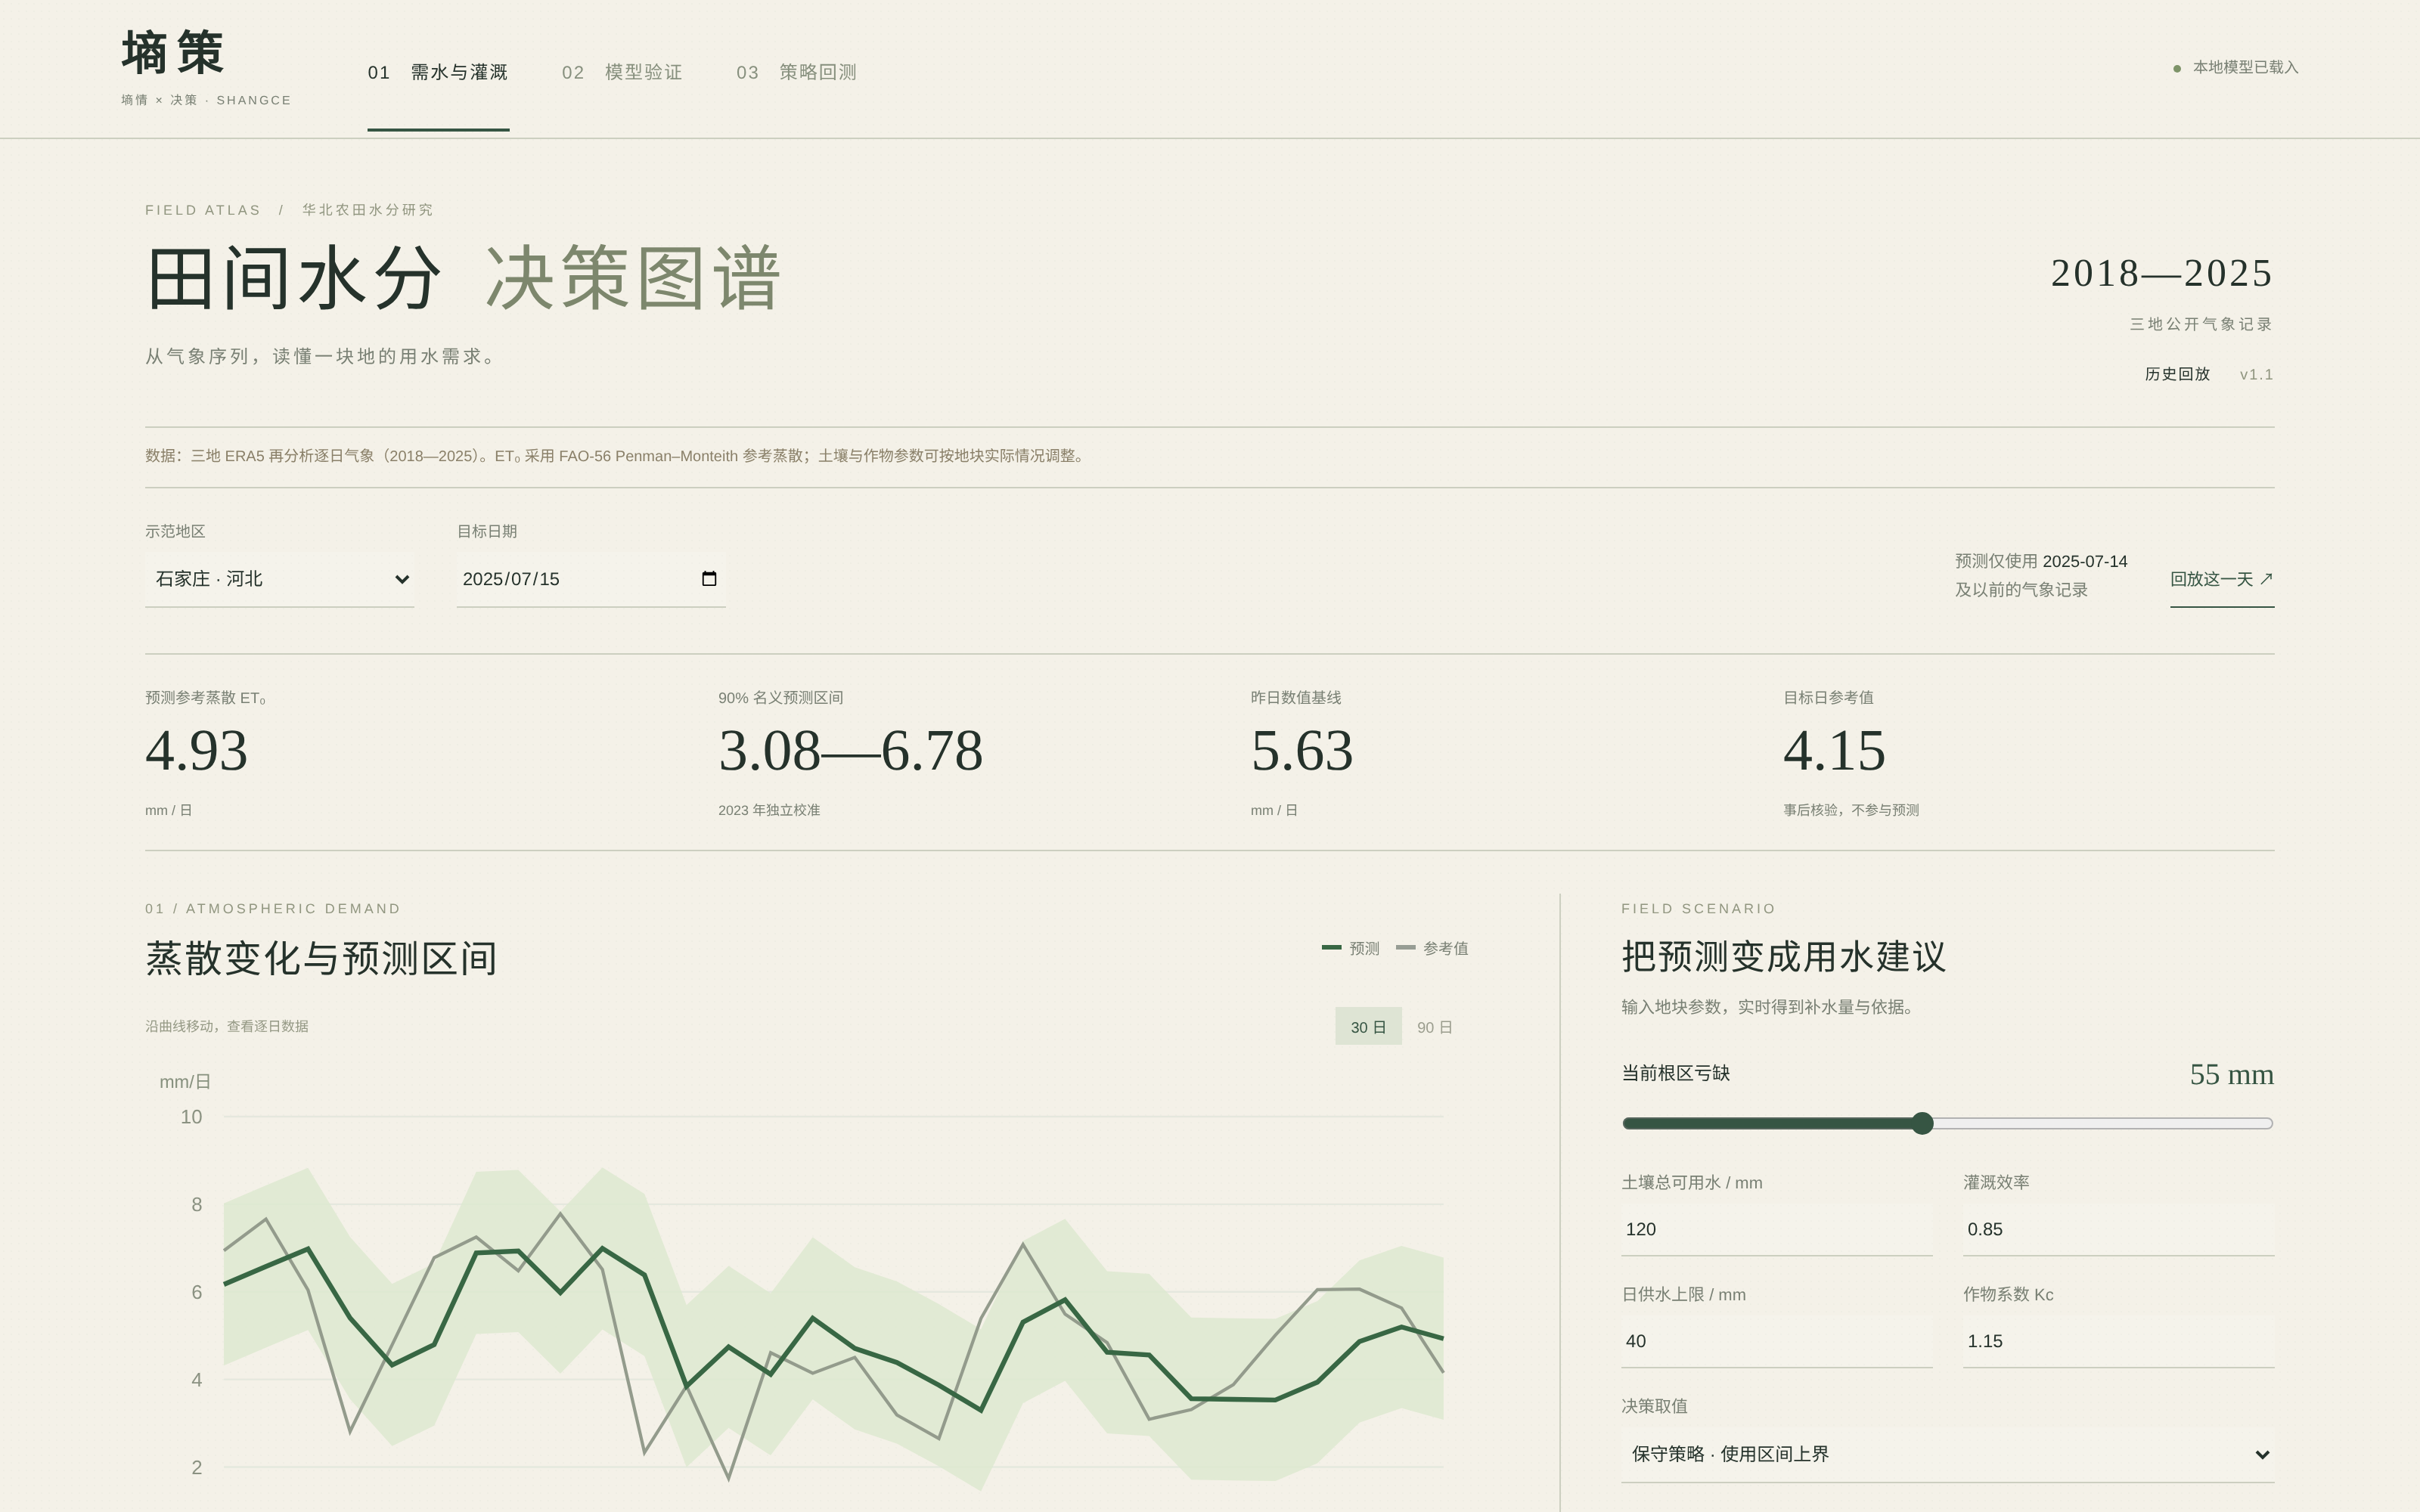
\includegraphics[width=.92\linewidth]{../results/screenshots/dashboard.png}
\caption{“需水与灌溉”视图：次日需水预测、预测区间与灌溉建议}\label{fig:ui}
\end{figure}

图\ref{fig:capacity}演示供水能力受限的情形：将日供水上限设为5 mm后，系统按上限给出5 mm毛灌溉量，提示供水能力不足，并显示补水后的预计亏缺。

\begin{figure}[H]\centering
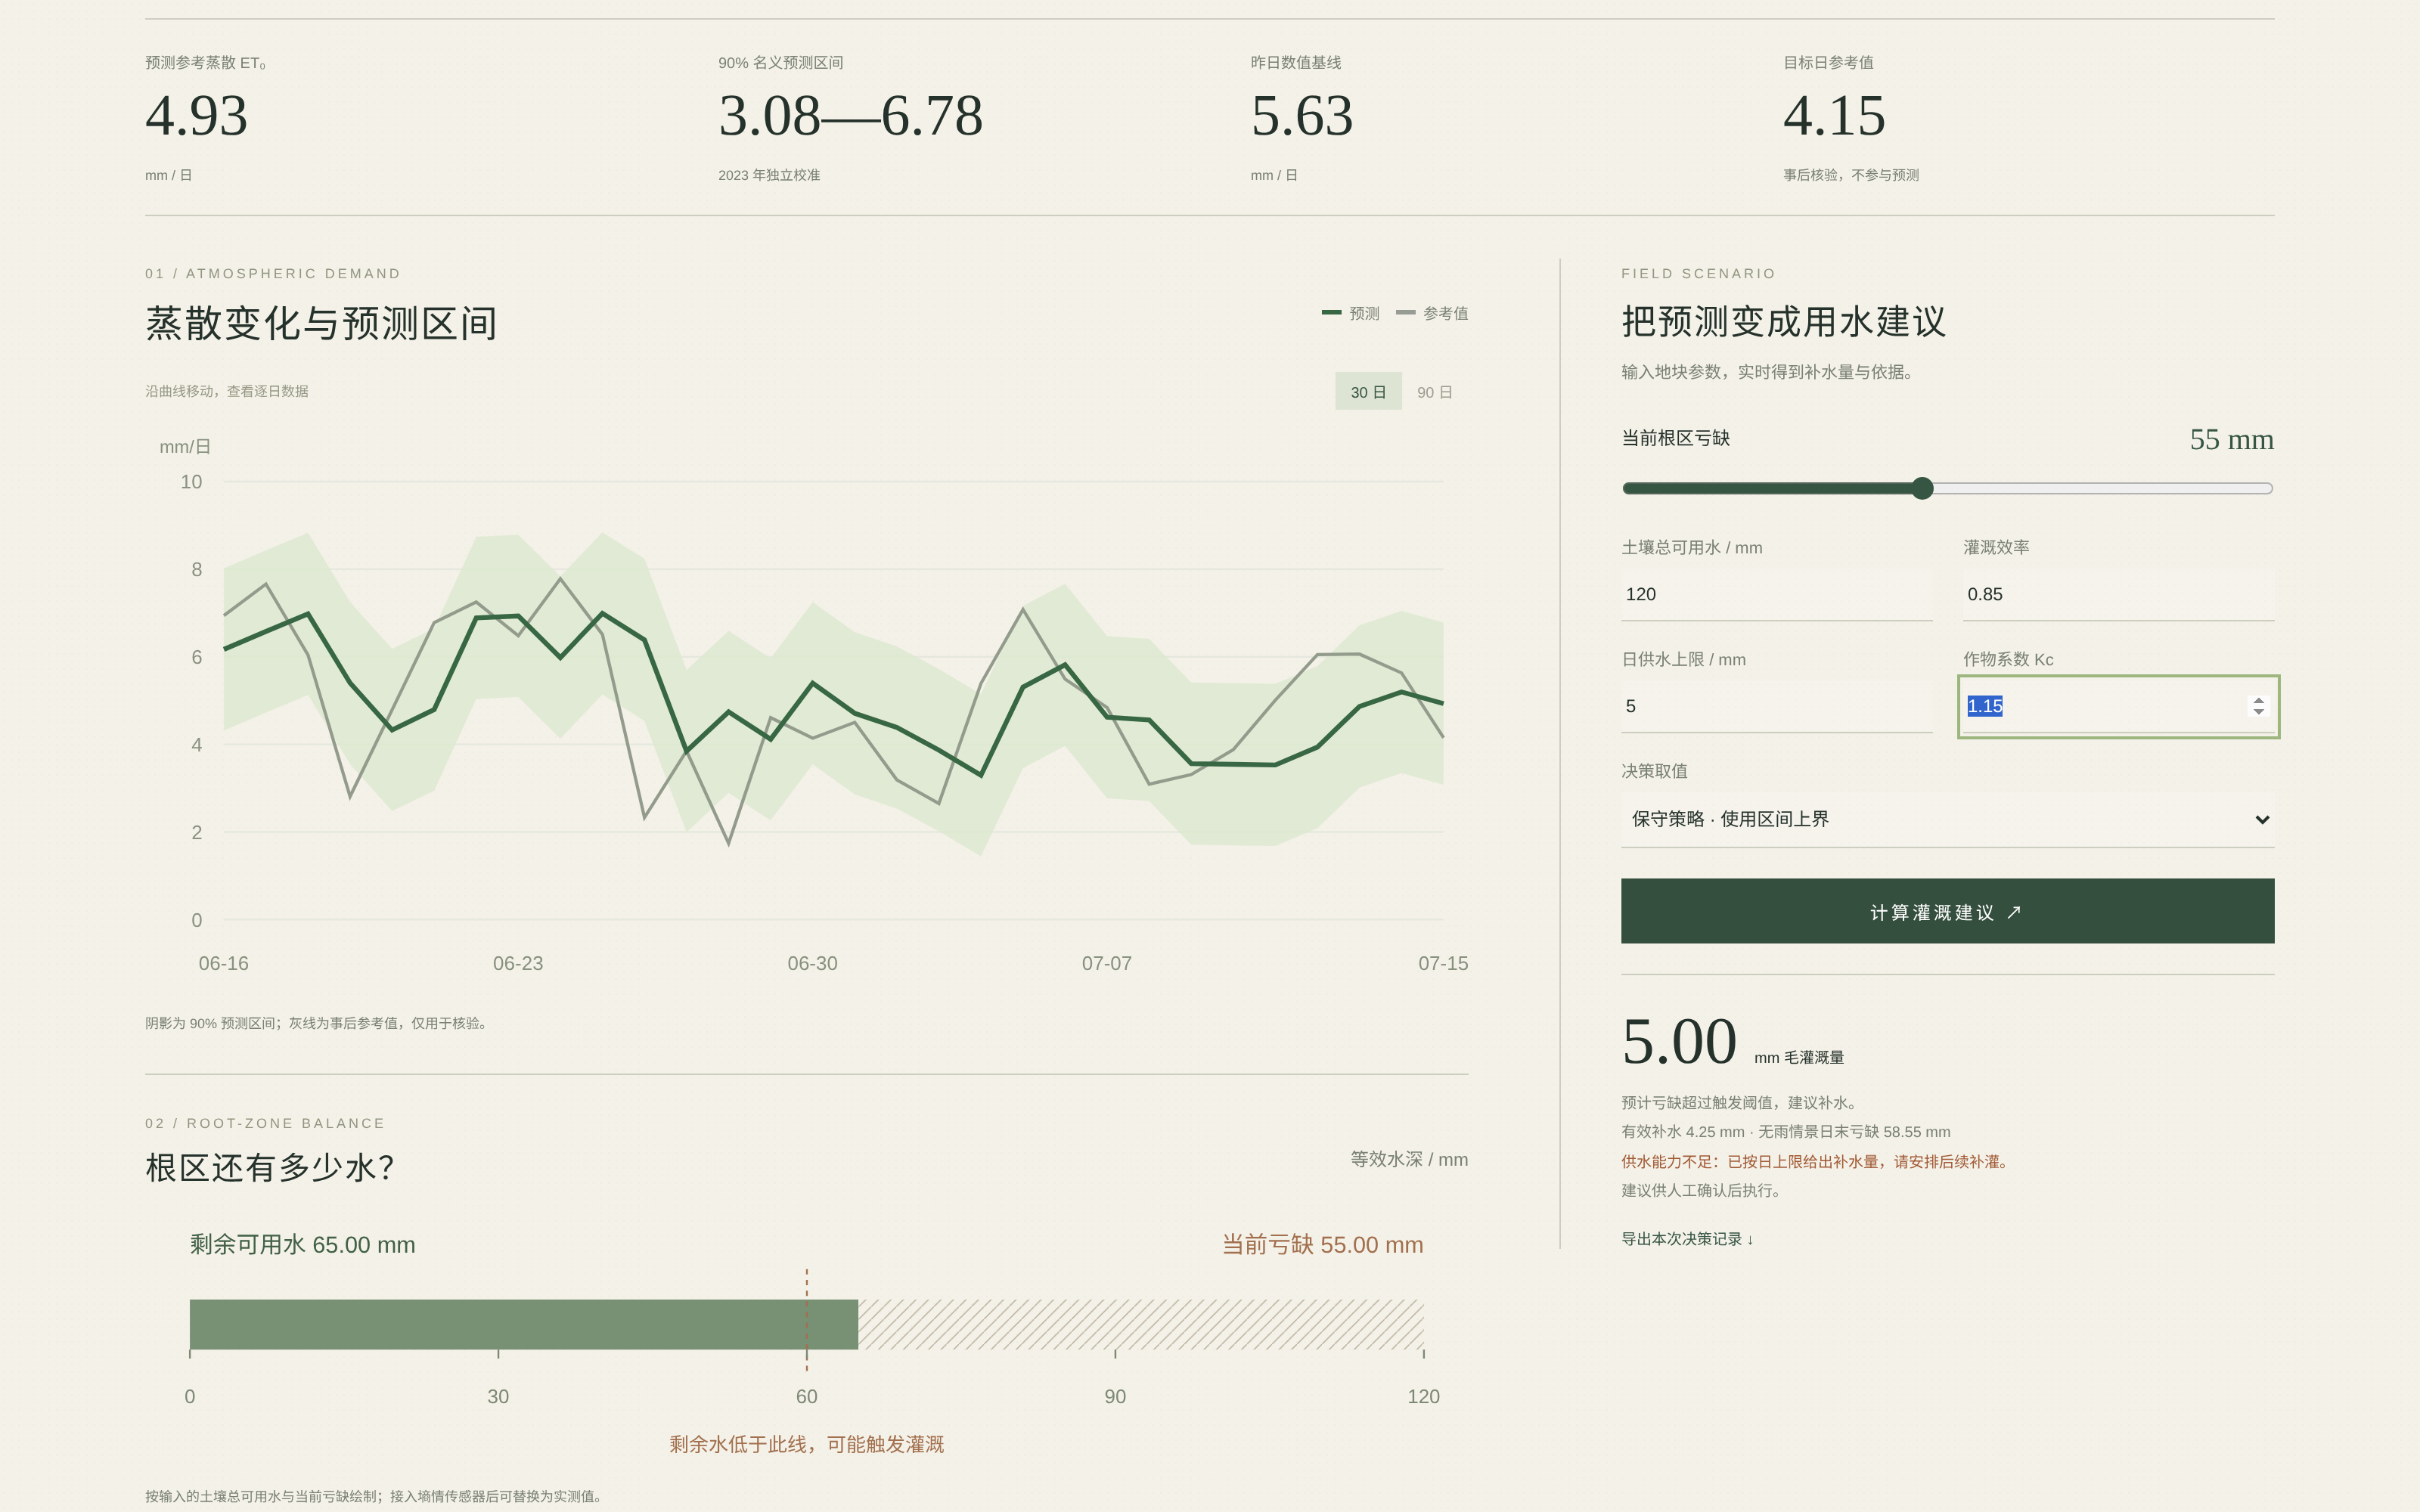
\includegraphics[width=.92\linewidth]{../results/screenshots/capacity.png}
\caption{供水上限为5 mm时的建议结果与能力不足提示}\label{fig:capacity}
\end{figure}

\subsubsection{测试与质量保障}
\begin{itemize}
\item \textbf{核心测试（9项，全部通过）}：未来数据扰动不改变特征、区间分位数计算、水量守恒、阈值边界、供水上限、非有限数值拒绝等；
\item \textbf{浏览器测试（9项，全部通过）}：初始推理、能力不足提示、JSON导出与页面输入一致、模型表与策略表渲染、非法输入禁止导出及恢复、手机布局无横向溢出、无未捕获异常；
\item \textbf{交付核验（61项，全部通过）}：从CSV重算MAE、RMSE、$R^2$与覆盖率，逐日水量汇总与180组季节结果一致，原始输入哈希匹配。
\end{itemize}

\clearpage\section{应用成效}\label{sec:results}
\subsection{成果展示}
\subsubsection{功能实现情况}
系统已完整实现表\ref{tab:requirements}中的全部功能需求：选择地区与日期即可回放任一测试日的次日需水预测、90\%预测区间、昨日值基线和事后参考值；输入土壤与设备参数后实时给出是否灌溉、毛灌溉量、净补水量和补水后预计亏缺；供水不足时自动提示；每次结果可导出为JSON决策记录。“模型验证”与“策略回测”视图集中展示本章的主要实验结果（图\ref{fig:evidence-ui}）。

\begin{figure}[H]\centering
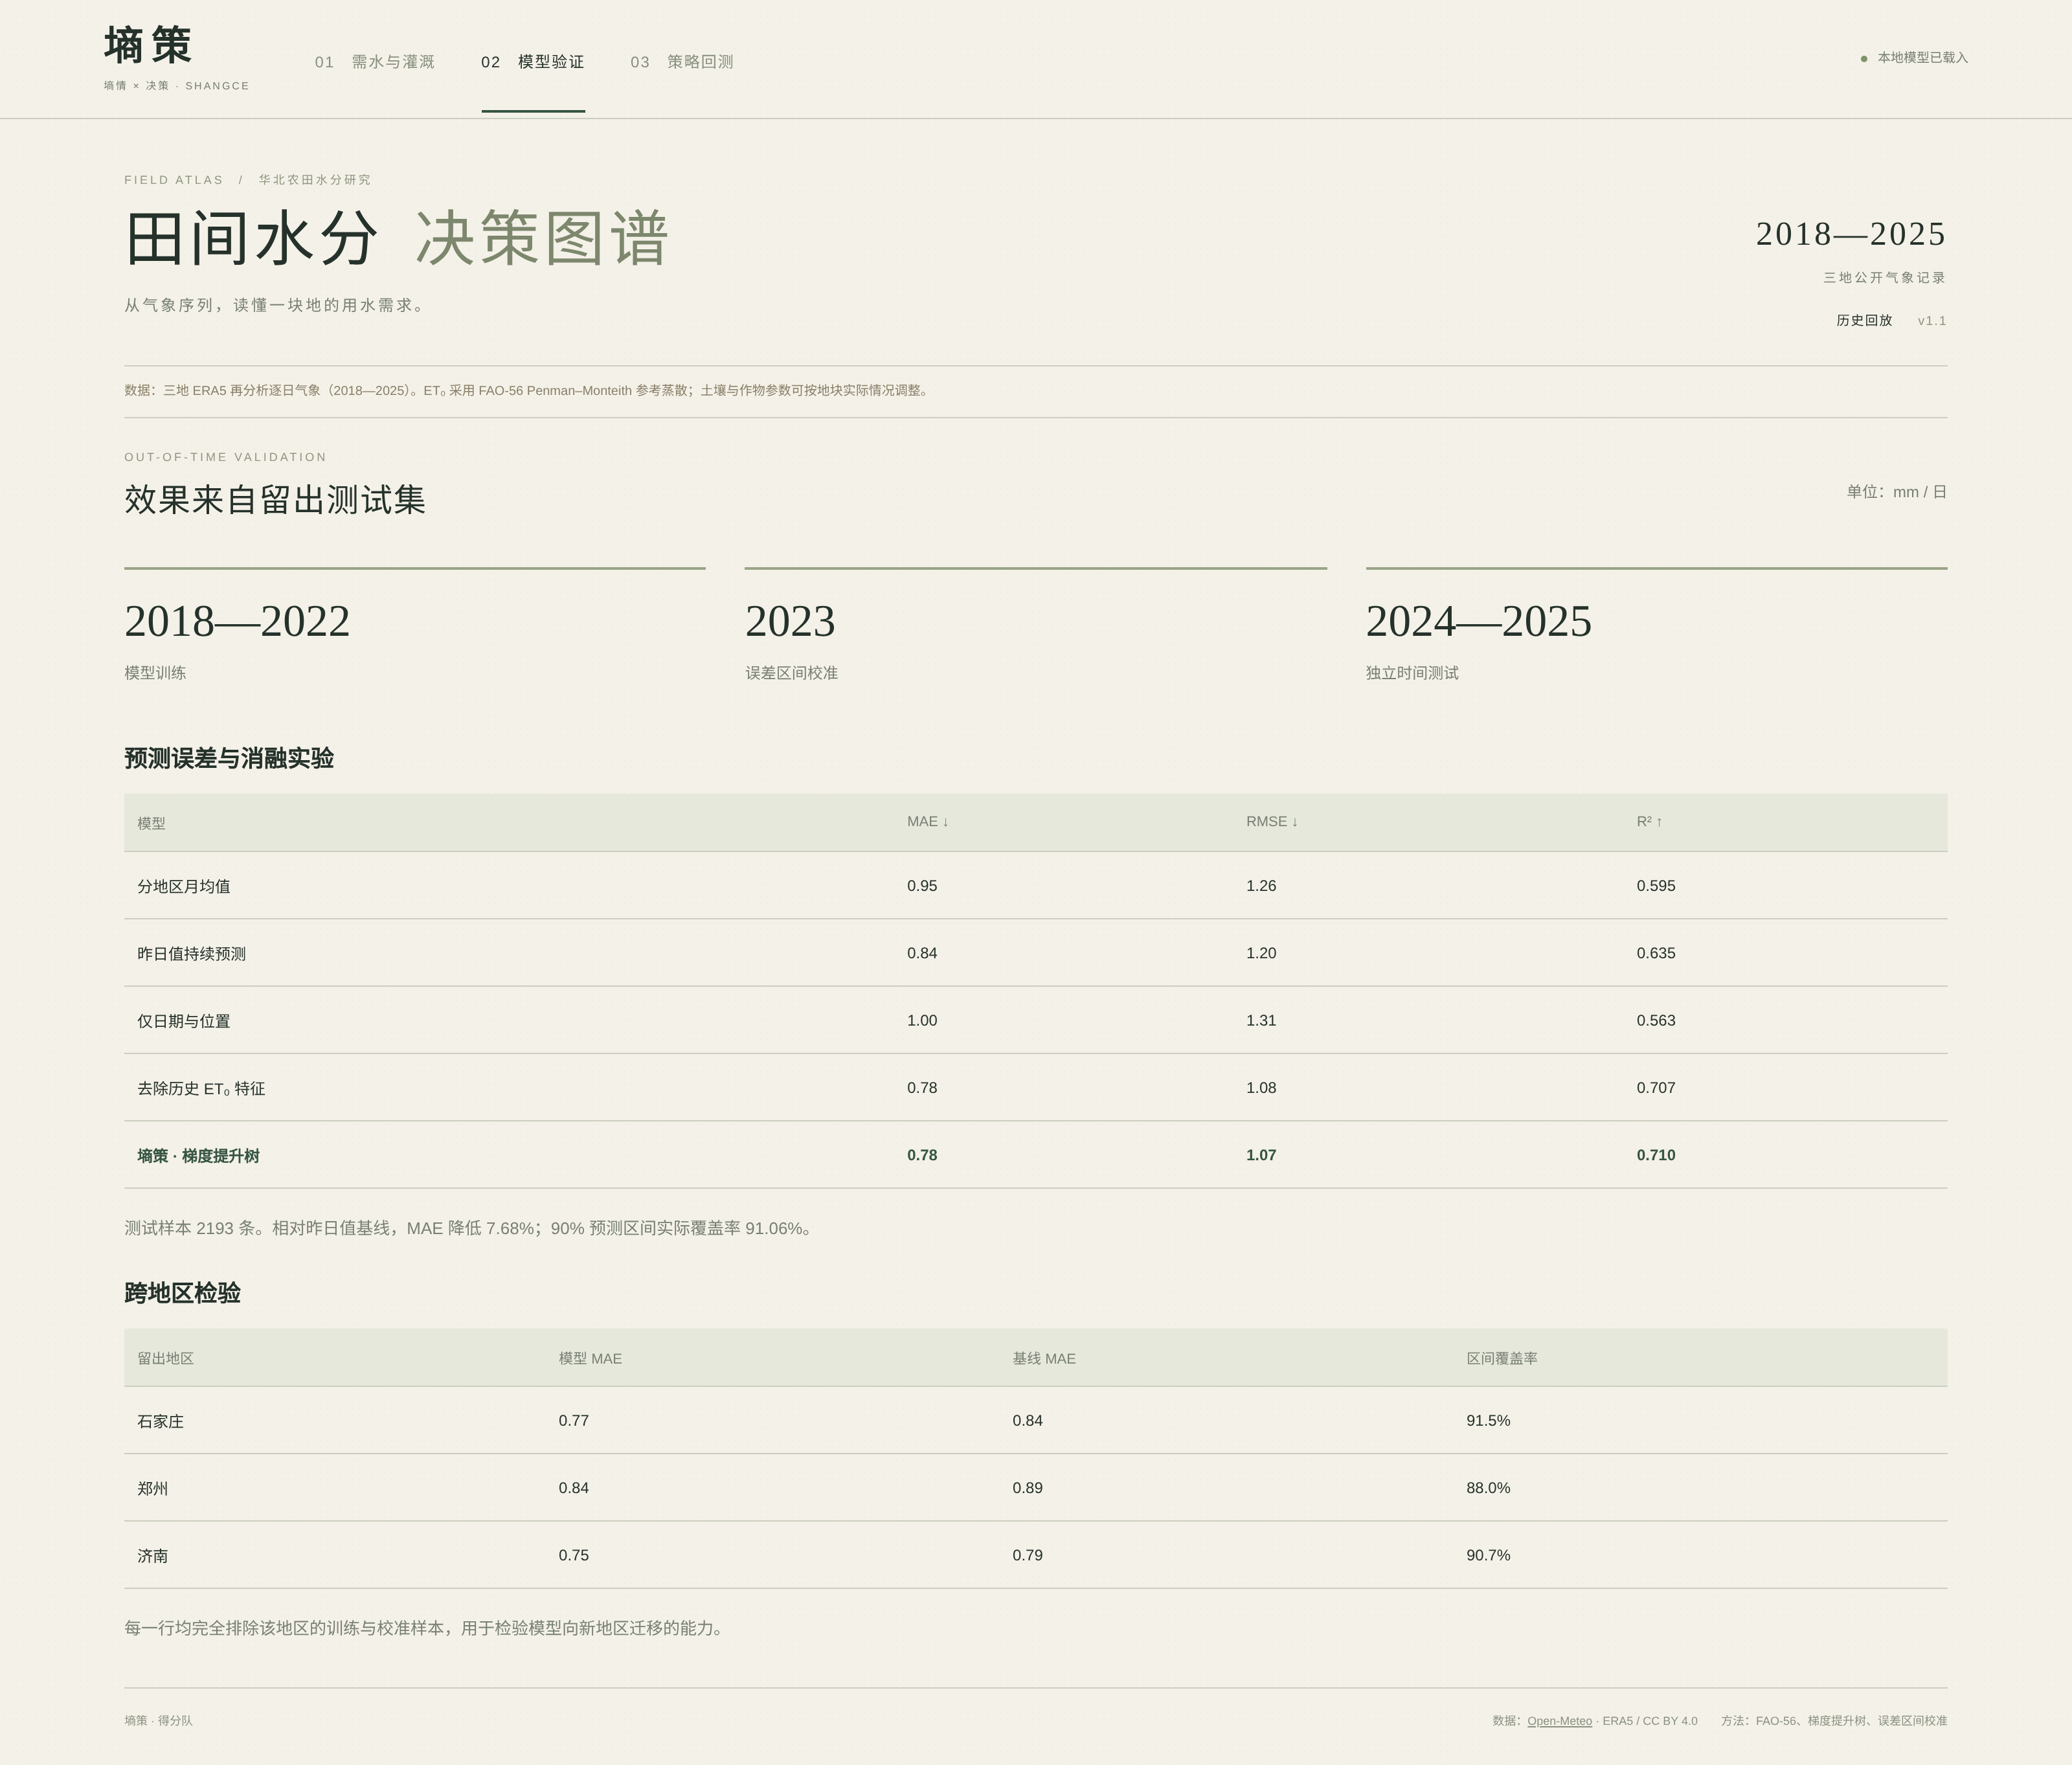
\includegraphics[width=.49\linewidth,height=.42\textheight,keepaspectratio]{../results/screenshots/evidence.png}\hfill
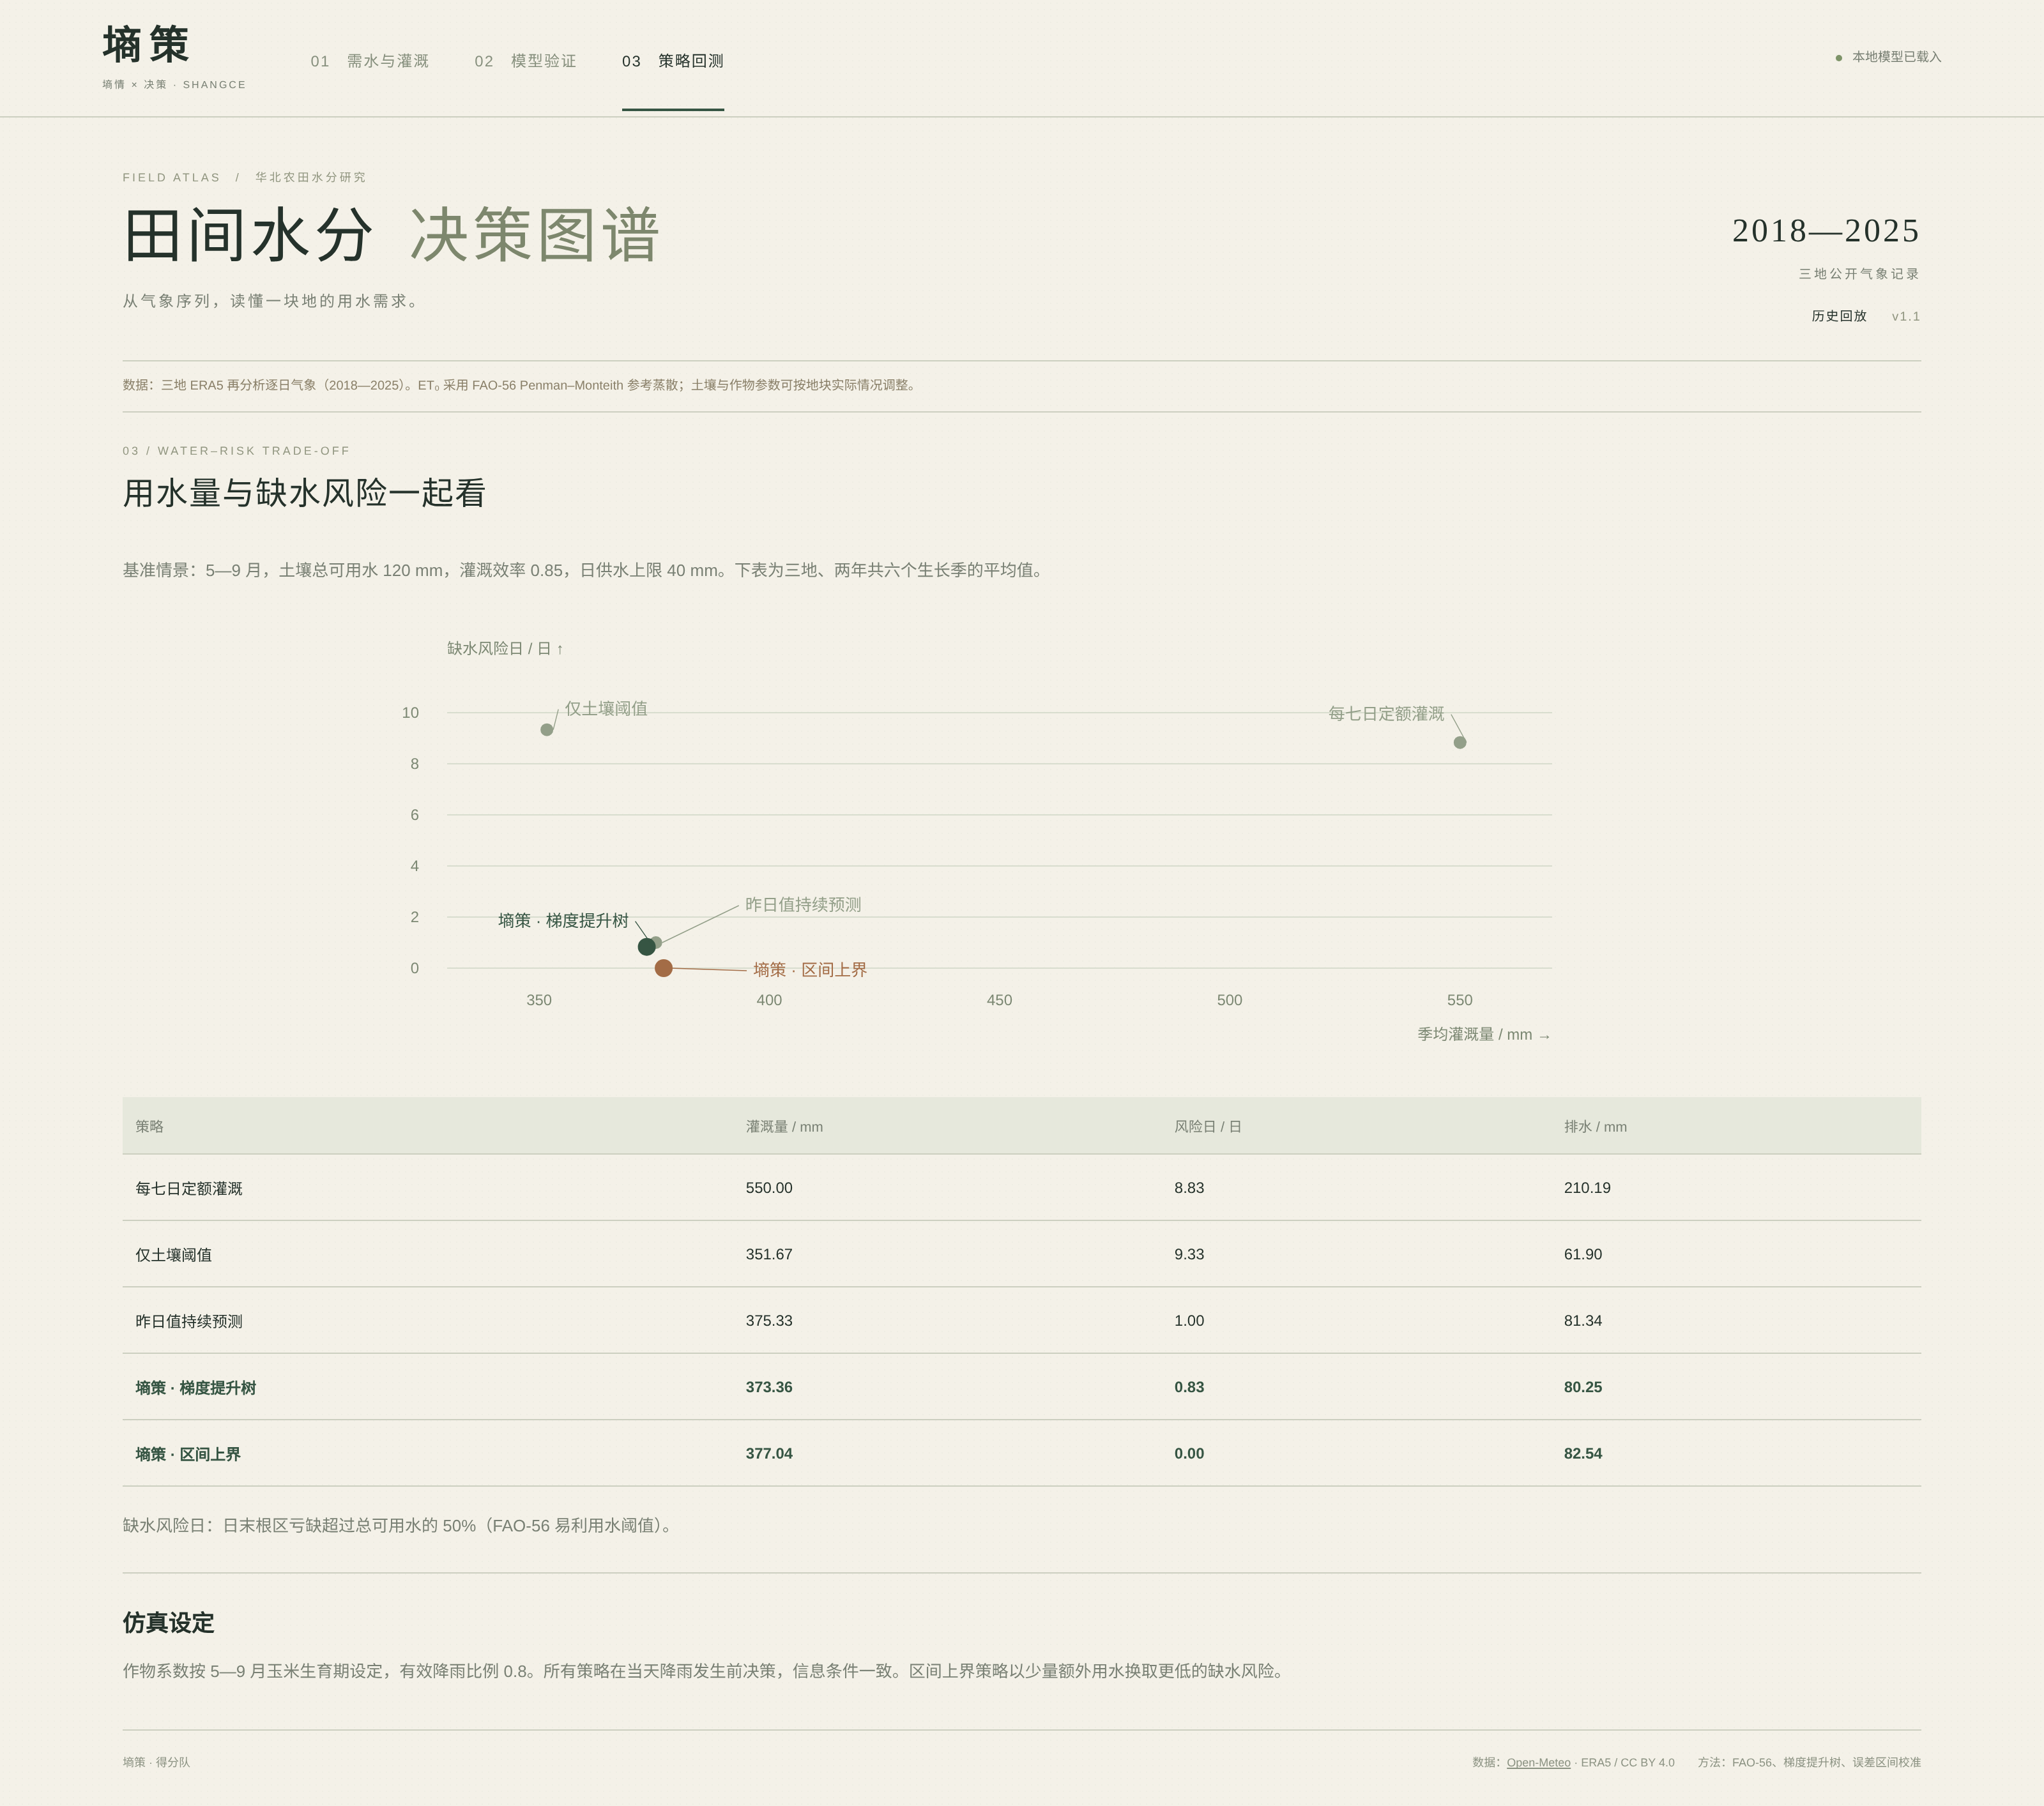
\includegraphics[width=.49\linewidth,height=.42\textheight,keepaspectratio]{../results/screenshots/simulation.png}
\caption{“模型验证”（左）与“策略回测”（右）视图}\label{fig:evidence-ui}
\end{figure}

\subsubsection{评价指标定义}
对标签$y_i$与预测$\widehat y_i$：
\begin{align}
\MAE&=\frac{1}{n}\sum_{i=1}^n|y_i-\widehat y_i|,\qquad
\RMSE=\sqrt{\frac{1}{n}\sum_{i=1}^n(y_i-\widehat y_i)^2},\\
R^2&=1-\frac{\sum_i(y_i-\widehat y_i)^2}{\sum_i(y_i-\bar y)^2}.
\end{align}
区间评价采用经验覆盖率与平均宽度：
\begin{equation}
\widehat{\mathrm{Cov}}=\frac1n\sum_i\mathbf1(y_i\in[L_i,U_i]),\qquad
\bar\ell=\frac1n\sum_i(U_i-L_i).
\end{equation}
误差单位均为mm/日。覆盖率与宽度需要同时报告：区间过宽会使上界策略过度灌溉，过窄则在高需水期失去保护作用。

\subsection{预测精度}
\datatable{overall}{完整模型与对照方法的时间留出测试结果}{tab:overall}{三地2024—2025年共2193条样本，所有方法在测试期均未调参。}

如表\ref{tab:overall}所示，完整模型的MAE为0.7757 mm/日，在五种方法中最低，较昨日值基线（0.8403 mm/日）降低
\begin{equation}
100\%\times\left(1-\frac{0.775680}{0.840251}\right)=7.68\%,
\end{equation}
RMSE由1.1994降至1.0688 mm/日，$R^2$由0.6352提高到0.7103。仅用日期与位置的模型MAE为0.9951 mm/日，甚至不如地区月均值，说明完整模型的优势主要来自近期多变量气象信息，而非模型复杂度本身。

对两种方法逐日绝对误差之差，按日期平均三地后以14日为块做1000次块自助重采样，得到MAE差值的95\%区间为[0.0332, 0.0965] mm/日，区间不含0，表明完整模型相对昨日值的改进是稳定的，而非偶然波动。

\datafigure{residual.pdf}{测试期预测散点与残差分布（残差=预测−参考）}{fig:residual}

图\ref{fig:residual}显示预测值紧密分布在1:1线两侧。残差均值为$-0.087$ mm/日，整体略有低估；绝对误差中位数0.547 mm/日，90\%与95\%分位数分别为1.791和2.253 mm/日。完整模型在54.72\%的测试日误差小于昨日值。

\subsection{分地区与消融分析}
\datatable{site_year}{完整模型的地区—年份分组表现}{tab:siteyear}{该表模型训练时包含三地，属于分组评价。}

三地两年的六个分组中，模型MAE全部低于昨日值（表\ref{tab:siteyear}）。改进最明显的是郑州2024年（0.749对0.873，降低14.2\%）和济南2024年（降低9.5\%）；郑州2025年改进最小（0.896对0.905），且覆盖率为89.04\%，略低于名义水平，是后续优化需要关注的分组。

消融实验中，去除全部历史ET\textsubscript{0}特征后MAE仅由0.7757升至0.7800 mm/日。这说明历史气温、辐射、湿度、风速等原始变量已包含参考蒸散的大部分信息，模型并不依赖平台计算的历史ET\textsubscript{0}，这有利于今后改用地面气象站数据作为输入。

\subsection{预测区间的覆盖与季节诊断}
测试期名义90\%区间的整体经验覆盖率为91.06\%，平均宽度3.61 mm/日；2193条样本中102条落在下界以下、94条高于上界，两侧失覆盖数量接近，区间没有系统性偏向。

\datafigure{seasonality.pdf}{分月MAE与经验覆盖率（虚线为90\%名义水平，棕色柱表示低于名义水平）}{fig:seasonality}

\datatable{monthly}{测试集分月误差、偏差与覆盖率}{tab:monthly}{偏差为预测减参考；覆盖率按该月三地两年合并计算。}

进一步按月份分解（图\ref{fig:seasonality}、表\ref{tab:monthly}），模型误差呈明显季节性：1月MAE仅0.303 mm/日，6月升至1.268 mm/日。由于区间采用全年统一的半宽$q$，冬季区间偏宽、覆盖率达100\%，而6月和7月覆盖率降至78.33\%和79.03\%。值得注意的是，即便在夏季，模型MAE仍低于昨日值（6月1.268对1.456），点预测的优势没有消失，问题出在区间宽度没有随季节自适应。这一发现直接指向第\ref{sec:outlook}章的改进方案：按季节或按预测误差尺度分别校准。

\datafigure{coverage_heatmap.pdf}{地区—月份经验覆盖率（\%）}{fig:heatmap}

图\ref{fig:heatmap}按地区细分了同一现象，三地夏季覆盖率均有不同程度下降，说明这是方法层面的共性问题，而非某一地区的数据异常。

\subsection{极端误差样本分析}
\datatable{worst}{绝对误差最大的八条测试记录}{tab:worst}{单位mm/日，按绝对误差从大到小排序。}

表\ref{tab:worst}列出误差最大的八条样本，集中在6月前后。例如郑州2024年6月16日，前一日参考值高达7.28 mm/日，当日骤降至1.81 mm/日，模型预测6.54 mm/日，虽已较昨日值有所修正，仍明显偏高。图\ref{fig:failure}显示该时段伴随明显降水过程。

\datafigure{failure_case.pdf}{郑州2024年6月误差案例窗口（降水为事后实况，不参与预测）}{fig:failure}

这类误差源于“仅凭历史信息难以预知次日天气突变”。在实际部署中接入次日天气预报（降水概率、云量、气温预报）作为输入，是降低此类误差最直接的手段。

\subsection{跨地区迁移}
\datatable{transfer}{完全留出目标地区的迁移检验}{tab:transfer}{每次在其余两地训练与校准，目标地区不参与这两个阶段。}

在完全没见过目标地区数据的条件下，三地点预测MAE均低于该地昨日值基线，石家庄、郑州、济南分别降低8.4\%、5.3\%和5.5\%；石家庄与济南的区间覆盖率保持在90\%以上，郑州为87.96\%。这表明模型具备向相似气候区推广的潜力；部署到新地区时，可尝试用当地一年数据重新校准区间以提高覆盖可靠性，这一做法有待在新地区实测验证。

\subsection{灌溉策略仿真}
\datatable{central}{基准情景下五种策略的六季平均结果}{tab:central}{TAW=120 mm、$\eta=0.85$，其余参数见表\ref{tab:assumptions}。}

表\ref{tab:central}给出基准情景下的结果。与定额日历相比，三种预测型策略的季均用水减少约31\%\,$\sim$\,32\%，风险日从8.83日降至1日及以下。与只看当前墒情的阈值策略相比，预测型策略多用约22\,$\sim$\,25 mm水，但仿真风险日从9.33日降至0\,$\sim$\,1日，说明“提前看一天”可以明显减少模型中的缺水风险日。AI区间上界策略在基准情景六个生长季中均未出现风险日，季均用水377.04 mm，仅比AI点预测多3.7 mm。

\datafigure{season_trace.pdf}{郑州2024年基准情景下的日末亏缺与累计灌溉（上图虚线为60 mm触发线）}{fig:trace}

逐日轨迹（图\ref{fig:trace}）显示，墒情阈值策略要等亏缺越过触发线后才补水，在高需水日多次短暂越线；预测型策略在越线前一天提前补水，其中上界策略的亏缺曲线全季位于触发线下方。累计用水曲线呈阶梯状，三种策略的季节总量相差不大，差别主要体现在补水时机上。

\datatable{six_seasons}{基准情景中点预测与上界策略的逐季结果}{tab:seasons}{用水为单季毛灌溉量（mm），风险为单季风险日数。}

\datafigure{tradeoff_all.pdf}{全部180组仿真的用水量—风险日分布（每种策略36个环境情景）}{fig:alltradeoff}

\datatable{paired}{AI区间上界策略相对各参照策略的环境内配对比较}{tab:paired}{差值为上界策略减参照，最后一列为36个情景中风险日减少/相同/增加的次数。}

为排除土壤与效率差异的干扰，表\ref{tab:paired}在每个环境情景内配对比较。相对于AI点预测，上界策略平均多用5.65 mm水，平均减少1.25个风险日，36个情景中27个风险更低、9个持平、0个更高；相对于墒情阈值策略，36个情景全部降低风险，平均减少11.25个风险日。上界策略为使用者提供了一个明确的“以少量用水换取更低风险”的选项。

\subsection{敏感性分析}
\datafigure{soil_sensitivity.pdf}{效率0.85时不同TAW下的六季平均用水与风险日}{fig:sensitivity}

图\ref{fig:sensitivity}和附录表\ref{tab:allsensitivity}显示：土壤储水越小（TAW=80 mm），各策略风险越高，不确定性信息的价值越突出——此时上界策略仍保持0风险日，而点预测为2.00日。灌溉效率由0.85降为0.70时，补足同样亏缺所需毛水量上升，40 mm日上限更容易成为约束。在全部6种“容量—效率”组合中，上界策略的风险日始终是五种策略中最低的（0\,$\sim$\,0.17日）；而AI点预测仅在基准组合中风险日低于昨日值，在其余5种组合中略高（差值0.17\,$\sim$\,0.67日）。这说明点预测精度的小幅提升不一定转化为更低的缺水风险，把误差区间纳入决策才是稳定降低风险的关键，这也印证了本作品“把预测误差放进灌溉决策”的设计思路。

\subsection{效益分析}
\textbf{节水与稳产潜力。}在6种“容量—效率”组合下（各为三地两年平均），AI区间上界策略相对于定额日历灌溉节约用水11\%\,$\sim$\,37\%（基准情景31.4\%），同时风险日不超过0.17日；相对于仅凭墒情阈值灌溉，以小幅增加用水换取缺水胁迫的大幅减少。这些结果来自统一参数下的仿真，实际节水与产量效益将通过田间影子运行和对照试验进一步验证（第\ref{sec:outlook}章）。

\textbf{社会效益。}系统完全离线运行、单次推理约11.5 ms、模型仅416 KiB，对硬件和网络没有要求，适合在基层农技站、合作社推广；界面直观展示“为什么要灌、为什么灌这么多”，有助于把科学灌溉方法传递给农户。

\textbf{教学与科研效益。}系统可作为农业水利、智慧农业课程的教学工具，学生能在同一天气条件下改变土壤、作物与设备参数，直观理解FAO-56水量平衡；完整开放的数据、代码与逐日结果也便于他人复现与扩展研究。

\clearpage\section{总结与展望}\label{sec:outlook}
\subsection{经验总结}
\subsubsection{主要成果}
本作品围绕“次日需水预测如何可信地进入灌溉决策”这一问题，完成了从公开数据到可交互决策工具的完整链条：
\begin{enumerate}
\item 基于三地8年ERA5逐日气象构建49维时间安全特征，梯度提升树次日参考蒸散预测MAE为0.7757 mm/日，较昨日值基线降低7.68\%，$R^2$达0.7103，块自助重采样表明改进稳定；
\item 以2023年独立数据完成共形校准，测试期90\%预测区间整体覆盖率91.06\%，并在留出地区检验中保持较好的迁移能力；
\item 将预测区间上界纳入FAO-56水量平衡规则，在180组生长季仿真中实现了缺水风险的稳定下降：基准情景风险日为0，相对墒情阈值策略在全部36个情景中均降低风险；
\item 实现了离线可运行的决策工作台，具备历史回放、参数交互、供水能力检查与决策记录导出功能，配套9项核心测试、9项浏览器测试和61项交付核验。
\end{enumerate}

\subsubsection{关键经验}
\textbf{时间边界是可信评估的前提。}特征窗口“先滞后、后聚合”、按年份切分训练—校准—测试，并用扰动测试自动检查，是避免信息泄漏、使指标可信的基础。

\textbf{分层评价比单一指标更有说服力。}点预测精度、区间覆盖与灌溉结果分层报告，才发现了“点预测略好不一定少缺水，区间上界才稳定降风险”这一对设计最有指导意义的结论。

\textbf{诊断比平均值更能指明方向。}全年91\%的覆盖率看似达标，分月诊断却揭示出夏季覆盖不足，为下一步改进提供了明确目标。

\subsubsection{不足之处}
\begin{table}[H]\centering\small
\caption{当前不足与改进措施}\label{tab:limitations}
\begin{tabularx}{\linewidth}{@{}p{.24\linewidth}XX@{}}\toprule
不足 & 影响 & 改进措施\\\midrule
区间半宽全年固定 & 6—7月覆盖率约78\%\,$\sim$\,79\%，冬季区间偏宽 & 分季节校准、共形分位数回归\cite{cqr}、自适应共形\cite{aci}\\
仅用历史气象输入 & 难以预知天气突变日 & 接入次日数值天气预报作为特征\\
使用再分析数据 & 再分析产品有发布延迟，网格尺度大于地块 & 改用实时预报与地面气象站数据\\
土壤与作物参数为设定值 & 仿真结果依赖参数选择 & 结合墒情传感器与当地农技资料标定\\
日尺度水桶模型 & 不表达分层入渗与日内胁迫 & 引入AquaCrop等作物模型\cite{aquacrop}\\
示范区为三个相邻地区 & 气候类型覆盖有限 & 扩展到西北、东北等不同气候区\\\bottomrule
\end{tabularx}
\end{table}

\subsection{未来规划}
\subsubsection{技术改进}
\textbf{（1）自适应预测区间。}按季节或按预测误差尺度分组校准，或采用共形分位数回归\cite{cqr}让区间宽度随天气条件变化；对存在分布漂移的时间序列，引入自适应共形推断\cite{aci}在线调整覆盖水平，目标是使每个月份的覆盖率都接近名义水平。

\textbf{（2）融合天气预报。}将未来1\,$\sim$\,3天的气温、降水概率、云量和风速预报作为新特征，并在决策时扣减预报降雨，减少降雨当天提前灌溉的情况，同时将预测时效由次日扩展到未来三天，支持轮灌排班。

\textbf{（3）接入田间墒情。}对接土壤水分传感器，用实测数据替代用户输入的亏缺值，并以“预测—观测”偏差在线修正TAW与作物系数，形成“预测—灌溉—观测—修正”的闭环。

\textbf{（4）多地块联合调度。}在共享水源和管网容量约束下，扩展为多地块轮灌优化，按缺水风险排序分配有限的供水能力。

\subsubsection{验证与推广计划}
\begin{table}[H]\centering\small
\caption{分阶段验证与推广计划}\label{tab:roadmap}
\begin{tabularx}{\linewidth}{@{}p{.16\linewidth}XX@{}}\toprule
阶段 & 主要任务 & 阶段目标\\\midrule
模型升级 & 实现自适应区间与天气预报特征，在新的外部年份上重新测试 & 夏季覆盖率接近90\%，天气转折日误差明显下降\\
影子运行 & 选择具备墒情与用水记录的试点地块，系统每日给出建议、农艺人员照常决策 & 积累建议与实际决策的对比数据，验证建议可执行性\\
对照试验 & 在可比地块开展系统建议与常规管理的对照 & 量化实际节水率、产量与能耗变化\\
推广应用 & 面向农技站、合作社和高校课程提供轻量部署版本 & 形成可复制的部署与培训方案\\\bottomrule
\end{tabularx}
\end{table}

\subsubsection{应用前景}
随着高标准农田建设和农业水价综合改革的推进，基层对“按需灌溉”工具的需求日益增长。墒策部署门槛低、计算过程透明，既可作为农技人员面向农户的灌溉参谋，也可嵌入灌区信息化平台，为墒情监测数据提供“下一步该怎么做”的决策出口；在教学场景中，可作为农业水利与智慧农业课程的实践工具。后续团队将按上述计划推进模型升级与试点验证，用田间数据持续检验和完善系统。

\clearpage\section{附录}
\subsection{数据资料}
\subsubsection{原始数据与来源}
原始数据为Open-Meteo历史天气接口返回的三地ERA5逐日气象（石家庄、郑州、济南，2018-01-01至2025-12-31，各2922天），以未改写的JSON保存在\file{inputs/weather/}，请求URL、获取时间与SHA-256哈希记录在\file{inputs/provenance.json}。数据按CC BY 4.0许可使用并注明来源\cite{om,license}。

\subsubsection{处理后数据}
\begin{table}[H]\centering\small
\caption{主要数据文件}\label{tab:files}
\begin{tabularx}{\linewidth}{@{}p{.42\linewidth}X@{}}\toprule
文件 & 内容\\\midrule
\file{results/weather_daily.csv} & 三地清洗后的逐日气象，8766行\\
\file{results/predictions.csv} & 2193条测试样本的预测、区间、基线与标签\\
\file{results/simulation_daily.csv} & 180组策略仿真的逐日水量记录，27540行\\
\file{results/simulation_scenarios.csv} & 180组季节汇总结果\\
\file{results/summary.json} & 实验汇总，界面与报告共用的数据源\\
\file{results/report_*.csv} & 分月、分地区年份、极端误差与敏感性统计\\\bottomrule
\end{tabularx}
\end{table}

\subsubsection{主要符号}
\begin{longtable}{@{}p{.19\linewidth}p{.19\linewidth}p{.54\linewidth}@{}}
\caption{主要符号及含义}\label{tab:symbols}\\\toprule
符号 & 单位 & 含义\\\midrule\endfirsthead
\toprule 符号 & 单位 & 含义\\\midrule\endhead
$s,t$ & — & 地区与目标日索引\\
$x_{s,t}$ & — & 49维模型输入\\
$y_{s,t}$ & mm/日 & 参考蒸散标签\\
$\widehat{\mathrm{ET}}_{0,t}$ & mm/日 & 模型点预测\\
$q$ & mm/日 & 校准残差分位数（区间半宽）\\
$L_t,U_t$ & mm/日 & 预测区间下界、上界\\
$K_{c,t}$ & — & 作物系数\\
$\mathrm{TAW}$ & mm & 根区总可用水\\
$\mathrm{RAW}$ & mm & 易利用水阈值，$p\,\mathrm{TAW}$\\
$D_t$ & mm & 决策前根区亏缺\\
$D_t^*$ & mm & 预计亏缺\\
$p,\beta$ & — & 触发比例、回填目标比例\\
$\eta$ & — & 灌溉效率\\
$C$ & mm/日 & 日毛灌溉上限\\
$I_t,I_t^{\rm net}$ & mm & 毛灌溉量、净补水量\\
$P_t,\rho$ & mm、— & 日降水、有效降水比例\\
$Q_t,\mathcal U_t$ & mm & 排水量、未满足需水量\\
$W,S$ & mm、日 & 季节毛灌溉量、缺水风险日\\\bottomrule
\end{longtable}

\subsection{代码与模型}
\subsubsection{代码结构}
\begin{table}[H]\centering\small
\caption{工程目录}\label{tab:code}
\begin{tabularx}{\linewidth}{@{}p{.34\linewidth}X@{}}\toprule
路径 & 说明\\\midrule
\file{src/pipeline.py} & 数据读取与校验、特征构造、训练、共形校准、对照、迁移检验与策略仿真\\
\file{src/agro.py} & FAO-56水量平衡、灌溉建议、参数校验与独立公式核验\\
\file{app/} & 本地推理服务（\texttt{server.py}）与交互界面\\
\file{models/shangce.joblib} & 已训练模型、特征列表、校准分位数与时间截止信息\\
\file{tests/test_core.py} & 核心单元测试\\
\file{scripts/} & 数据获取、报告图表生成、浏览器检查与交付核验脚本\\\bottomrule
\end{tabularx}
\end{table}

\subsubsection{运行与复现}
环境为Python 3.12，核心依赖NumPy 2.2.6、pandas 2.3.3、scikit-learn 1.7.2、joblib 1.5.2，完整版本见\file{requirements.lock.txt}。在工程根目录执行：
\begin{lstlisting}
python3 -m venv .venv
.venv/bin/python -m pip install -r requirements.txt
.venv/bin/python -m src.pipeline          # 训练、评估与仿真
.venv/bin/python -m pytest -q             # 核心测试
.venv/bin/python scripts/report_analysis.py   # 诊断图表
.venv/bin/python app/server.py --port 8765    # 启动系统
\end{lstlisting}
浏览器访问\texttt{http://127.0.0.1:8765}即可使用。原始数据随工程提供，训练与推理无需联网。

\subsubsection{核心算法片段}
以下为特征构造中保证时间边界的关键实现（节选自\file{src/pipeline.py}）：
\begin{lstlisting}[language=Python]
def features(weather):
    all_frames=[]
    for site,d in weather.groupby('site',sort=True):
        d=d.sort_values('date').copy()
        d['sin']=np.sin(2*np.pi*d.date.dt.dayofyear/365.25)
        d['cos']=np.cos(2*np.pi*d.date.dt.dayofyear/365.25)
        # 每行日期为预测目标日，只使用该日之前的历史数据
        for col in PARAMS+['et0']:
            for lag in [1,2,3,7]: d[f'{col}_lag{lag}']=d[col].shift(lag)
            d[f'{col}_mean7']=d[col].shift(1).rolling(7,min_periods=7).mean()
\end{lstlisting}

\subsubsection{一个可复核的决策算例}
系统导出的一条实际决策记录：济南，目标日2025年7月15日，上界策略参考蒸散8.0243 mm/日，输入$D=90$ mm、TAW=120 mm、$K_c=1.15$、$\eta=0.85$、$C=5$ mm。代入式\eqref{eq:projected}—\eqref{eq:capacity}：
\begin{align}
D^*&=90+1.15\times8.0243=99.2280\ \mathrm{mm},\\
I^{\rm req}&=(99.2280-30)/0.85=81.4447\ \mathrm{mm},\\
I&=\min(5,81.4447)=5\ \mathrm{mm},\qquad I^{\rm net}=0.85\times5=4.25\ \mathrm{mm},\\
D^{\rm after}&=99.2280-4.25=94.9780\ \mathrm{mm}.
\end{align}
导出结果中预计亏缺为94.9780 mm，标记\texttt{capacity\_limited=true}，与手工计算一致，表明当日供水能力远不足以回填至目标亏缺。

\subsubsection{容量与效率组合的完整结果}
表\ref{tab:allsensitivity}列出全部30种“TAW—效率—策略”组合的六季平均结果。逐地区、逐年份的180组结果见工程文件：

\file{results/simulation_scenarios.csv}

\begin{longtable}{rrlrr}
\caption{全部容量与效率组合的六季平均结果}\label{tab:allsensitivity}\\\toprule
TAW/mm & $\eta$ & 策略 & 毛灌溉量/mm & 风险日/日\\\midrule\endfirsthead
\toprule TAW/mm & $\eta$ & 策略 & 毛灌溉量/mm & 风险日/日\\\midrule\endhead
80 & 0.70 & AI点预测 & 479.15 & 2.00 \\
80 & 0.70 & 定额日历 & 550.00 & 35.17 \\
80 & 0.70 & 昨日值 & 490.51 & 1.83 \\
80 & 0.70 & 墒情阈值 & 469.02 & 14.67 \\
80 & 0.70 & AI上界 & 488.40 & 0.00 \\
80 & 0.85 & AI点预测 & 394.60 & 2.00 \\
80 & 0.85 & 定额日历 & 550.00 & 24.17 \\
80 & 0.85 & 昨日值 & 403.95 & 1.83 \\
80 & 0.85 & 墒情阈值 & 386.25 & 14.67 \\
80 & 0.85 & AI上界 & 402.21 & 0.00 \\
120 & 0.70 & AI点预测 & 440.00 & 1.33 \\
120 & 0.70 & 定额日历 & 550.00 & 28.83 \\
120 & 0.70 & 昨日值 & 440.00 & 0.67 \\
120 & 0.70 & 墒情阈值 & 420.00 & 10.50 \\
120 & 0.70 & AI上界 & 446.67 & 0.17 \\
120 & 0.85 & AI点预测 & 373.36 & 0.83 \\
120 & 0.85 & 定额日历 & 550.00 & 8.83 \\
120 & 0.85 & 昨日值 & 375.33 & 1.00 \\
120 & 0.85 & 墒情阈值 & 351.67 & 9.33 \\
120 & 0.85 & AI上界 & 377.04 & 0.00 \\
160 & 0.70 & AI点预测 & 400.00 & 1.17 \\
160 & 0.70 & 定额日历 & 550.00 & 22.33 \\
160 & 0.70 & 昨日值 & 406.67 & 0.83 \\
160 & 0.70 & 墒情阈值 & 400.00 & 10.17 \\
160 & 0.70 & AI上界 & 406.67 & 0.00 \\
160 & 0.85 & AI点预测 & 346.67 & 0.33 \\
160 & 0.85 & 定额日历 & 550.00 & 3.17 \\
160 & 0.85 & 昨日值 & 346.67 & 0.17 \\
160 & 0.85 & 墒情阈值 & 333.33 & 8.33 \\
160 & 0.85 & AI上界 & 346.67 & 0.00 \\
\bottomrule
\end{longtable}


\subsection{其他材料}
\begin{itemize}
\item \textbf{演示视频}：系统实际运行录屏，展示历史回放、灌溉建议、供水限制、模型验证与策略回测全流程；
\item \textbf{答辩PPT}：作品背景、核心技术、实验结果、创新点与应用前景；
\item \textbf{佐证材料}：数据来源与完整性校验、模型运行与测试记录、系统功能截图；
\item \textbf{完整工程}：源码、原始数据、模型文件、逐日结果与复现脚本，按大赛要求上传至百度网盘。
\end{itemize}

\clearpage
\addcontentsline{toc}{section}{参考文献}
\begin{thebibliography}{99}\small
\bibitem{fao} Allen R G, Pereira L S, Raes D, Smith M. Crop evapotranspiration: Guidelines for computing crop water requirements[R]. FAO Irrigation and Drainage Paper 56. Rome: FAO, 1998.
\bibitem{pereira} Pereira L S, Allen R G, Smith M, Raes D. Crop evapotranspiration estimation with FAO56: Past and future[J]. Agricultural Water Management, 2015, 147: 4--20.
\bibitem{fereres} Fereres E, Soriano M A. Deficit irrigation for reducing agricultural water use[J]. Journal of Experimental Botany, 2007, 58(2): 147--159.
\bibitem{aquacrop} Steduto P, Hsiao T C, Raes D, Fereres E. AquaCrop---The FAO crop model to simulate yield response to water: I. Concepts and underlying principles[J]. Agronomy Journal, 2009, 101(3): 426--437.
\bibitem{era5} Hersbach H, Bell B, Berrisford P, et al. The ERA5 global reanalysis[J]. Quarterly Journal of the Royal Meteorological Society, 2020, 146(730): 1999--2049.
\bibitem{om} Open-Meteo. Historical Weather API[EB/OL]. [2026-10-13]. \url{https://open-meteo.com/en/docs/historical-weather-api}.
\bibitem{fan} Fan J, Yue W, Wu L, et al. Evaluation of SVM, ELM and four tree-based ensemble models for predicting daily reference evapotranspiration using limited meteorological data in different climates of China[J]. Agricultural and Forest Meteorology, 2018, 263: 225--241.
\bibitem{feng} Feng Y, Cui N, Gong D, Zhang Q, Zhao L. Evaluation of random forests and generalized regression neural networks for daily reference evapotranspiration modelling[J]. Agricultural Water Management, 2017, 193: 163--173.
\bibitem{friedman} Friedman J H. Greedy function approximation: A gradient boosting machine[J]. The Annals of Statistics, 2001, 29(5): 1189--1232.
\bibitem{xgb} Chen T, Guestrin C. XGBoost: A scalable tree boosting system[C]//Proceedings of the 22nd ACM SIGKDD International Conference on Knowledge Discovery and Data Mining. 2016: 785--794.
\bibitem{lgbm} Ke G, Meng Q, Finley T, et al. LightGBM: A highly efficient gradient boosting decision tree[C]//Advances in Neural Information Processing Systems 30. 2017: 3146--3154.
\bibitem{sklearn} Pedregosa F, Varoquaux G, Gramfort A, et al. Scikit-learn: Machine learning in Python[J]. Journal of Machine Learning Research, 2011, 12: 2825--2830.
\bibitem{vovk} Vovk V, Gammerman A, Shafer G. Algorithmic Learning in a Random World[M]. New York: Springer, 2005.
\bibitem{lei} Lei J, G'Sell M, Rinaldo A, Tibshirani R J, Wasserman L. Distribution-free predictive inference for regression[J]. Journal of the American Statistical Association, 2018, 113(523): 1094--1111.
\bibitem{conformal} Angelopoulos A N, Bates S. A gentle introduction to conformal prediction and distribution-free uncertainty quantification[EB/OL]. arXiv:2107.07511, 2021.
\bibitem{cqr} Romano Y, Patterson E, Cand\`es E. Conformalized quantile regression[C]//Advances in Neural Information Processing Systems 32. 2019.
\bibitem{aci} Gibbs I, Cand\`es E. Adaptive conformal inference under distribution shift[C]//Advances in Neural Information Processing Systems 34. 2021.
\bibitem{license} Open-Meteo. Licence[EB/OL]. [2026-10-13]. \url{https://open-meteo.com/en/licence}.
\end{thebibliography}
\end{document}
